%===================================== CHAP 7 =================================

\chapter{Results} \label{chapter_computational_study}

In this chapter, the results of the solution framework outlined in Chapter \ref{chapter_solution_approach} implemented with the numerical values for parameters computed in Chapter \ref{chapter_experimental_setup} run on the 2017/2018 season is presented. First, in Section \ref{sec:exact}, the optimal ex-post decisions are presented. Secondly, in Section \ref{sec:inexact}, the performance of the forecast-based optimization model for the FPL with the three different forecasting methods is presented. Finally, an ex-post analysis of the risk handling constraints is given. 

\newpar

The mathematical model is written in the modelling language Mosel and implemented in FICO\textsuperscript {\textregistered} Xpress Optimization Suite 8.3, using a HP EliteDesk 800 G3 DM 65W computer with Intel\textsuperscript{\textregistered} Core\textsuperscript{\texttrademark} i7-7700 3.6 GHz processor and 32 GB RAM. The operating system in use is Windows 10 Education 64-bit. The input data to the mathematical model is structured and pre-processed in the statistical programming language R. Further, the results obtained from the mathematical model include decisions on selected squad, starting line-up, substitution priority, number of penalized transfers, captain, vice-captain and whether a gamechip is used in a gameweek. These are written to CSV files, which are exported back to R to calculate how many points the team obtained. In the end, R is also used to make the data more presentable in form of tables and plots. 

\newpar

As mentioned in Section \ref{exp_setup_data}, the model is solved for the first 35 gameweeks of the 2017/2018 season. The transfer window closed after gameweek 26. Until then, 625 players had appeared in at least one game. Thus, the set consists of 625 players.

\section{Solution With Realized Points}\label{sec:exact}


Before the performance of the forecast-based optimization model for the FPLDP is examined, it is interesting to study the optimal solution ex-post. Firstly, the solution serves as a benchmark for the performance of the forecast-based optimization model for the FPLDP. Further, the optimal solution is compared to that of the top-performing manager, in order to see how close the best manager performs, and if there exists a potential for improvement. This section is divided into three parts. First, the initialization of sets and parameters is presented. Following is a discussion of the results obtained by the mathematical model using realized points for the 2017/2018 season. Secondly, the solution is more thoroughly examined to discuss whether the decisions are sensible or not. Finally, the solution is compared against the best performing human managers. 


\subsection{Initialization of parameters}    
%DEL1 

Following in Table \ref{tab:initializations_of_sets} and \ref{tab:initialization_of_parameters} are the initialization of parameters and sets used when the mathematical model is solved with realized points. 

\begin{table}[H]
\centering

\begin{tabular}{@{}lll@{}}
\toprule
Set           &   &                                                               \\ \midrule
$\mathcal{T}$ & - & 35 gameweeks.                                             \\
$\mathcal{P}$ & - & 625 players.                                              \\
$\mathcal{C}$ & - & 20 teams.                                                 \\
$\mathcal{L}$ & - & \{1, 2, 3\}, where 1 is first priority. \\
$\mathcal{T}_{FH}$ & - & Gameweek 1 to 21 is in the first half of the season. \\
$\mathcal{T}_{SH}$ & - & Gameweek 22 to 35 is in the second half of the season. \\
\bottomrule
\end{tabular}
\caption{Initialization of sets.}
\label{tab:initializations_of_sets}
\end{table}

\begin{table}[H] 
\tabcolsep=0.11cm
\centering
\begin{tabular}{@{}lll@{}}
\toprule
Parameters                       &   &                                                                                                \\ \midrule
$\mathlarger{\rho_{pt}}$ & - & Realized points for a player $p$ in a gameweek $t$. \\
$\epsilon$                       & - & Set to 0.1.                                                                     \\
$\kappa_{1}, \kappa_{2}, \kappa_{3} $                     & - & Set to 0.01, 0.001 and 0.0001, respectively.                                               \\
$C_{pt}^{B}$                     & - & Buy price collected from FPL homepage.  \\ 
$R$                              & - & 4 points deducted if number of free transfers is exceeded.       \\
$M^{K}$                          & - &  2 goalkeepers required in the selected squad.                                      \\
$M^{D}$                          & - &  5 defenders required in the selected squad.                         \\
$M^{M}$                          & - & 5 midfielders required in the selected squad.                                     \\
$M^{F}$                          & - & 3 forwards required in the selected squad.                                    \\
$M^{C}$                          & - & 3 players allowed to have from the same team.                                \\
$E$                              & - & 11 players required in the starting line-up.                              \\
$E^{K}$                          & - & 1 goalkeepers required in the starting line-up.                                       \\
$E^{D}$                          & - & 3 defenders required in the starting line-up.                  \\
$E^{M}$                          & - & 3 midfielders required in the starting line-up.                                 \\
$E^{F}$                          & - & 1 forward required in the starting line-up.                     \\
$B^{S}$                          & - & 100 million as starting budget.                                                                              \\
$\beta$                          & - & Set to 1.                                                                                  \\          
$\bar{\alpha}$                   & - & Set to 14.                                                                      \\

$\phi$                           & - & 3 players are substitutes.                                                         \\
$\phi^{K}$                       & - & 1 keeper among the substitutes.                                                          \\
$\overline{Q}$                   & - & 2 free transfers possible to accumulate over gameweeks.                                              \\
$\underline{Q}$                  & - & 1 free transfer given every gameweek.                                      \\ \bottomrule
\end{tabular}
\caption{Initialization of parameters.}
\label{tab:initialization_of_parameters}
\end{table}


All the parameters specifically stated in the rules of FPL are set accordingly. These include number of points deducted if the number of free transfers are surpassed, number of players in different position in both selected squad and starting line-up, maximum players from same team, starting budget and the restrictions on free transfers. The parameter in the objective function for vice-captain are set to 0.1, while for the substitution priority, $\kappa_{1}, \kappa_{2}, \kappa_{3}$ are set to 0.01, 0.001 and 0.0001, respectively. To tighten the formulation as much as possible, the parameters $\beta$ and $\alpha$ are set so to the smallest, but sufficiently high, value. $\beta$ is used in constraints \eqref{eq:subst} and \eqref{eq:free_hit_subst} in Chapter \ref{chapter_model_formulation} which concern the substitution priority. Considering that the variables adopted are binary, setting the value to 1 is reasonable. $\alpha$ is used in constraints \eqref{eq:trans_flow_illegal_transfers}, and is set to highest possible value for number of points-deducting transfers. As 1 free transfer is given each gameweek and the selected squad consists of 15 players, it is not possible to have more than 14 points-deducting transfers. Hence, the parameter $\alpha$ is set accordingly. 



\subsection{Problem Size}

Table \ref{tab:computational_statistics} displays the problem size of FPLDP with input data from the 2017/2018 season. The problem size is given before and after the function Presolve is run. This is a function integrated in Xpress Optimizer where its objectives are to reduce redundant variables, eliminate redundant constraints and remove linearly dependent constraints, which consequently reduces the complexity of the problem and improve the computing time. From the table it can be observed that the Presolve function is successful in eliminating variables, but the reduction of constraints is not that severe. A reason for this could be that most of the constraints are linearly independent, and that there is a limited presence of empty rows in the FPLDP. In addition, a large part of the variables $x_{pt}$, $x_{pt}^{freehit}$ and $y_{pt}$ are redundant, as many of them are defined even though only a few of them are used in the starting line-up and selected squad constraints. Thus, in order to reduce the solution time, an effort could have been put into reducing redundant variables in the procedure of implementation. However, since the model only has to be solved once, this is disregarded. 


\begin{table}[H]
\centering
\begin{tabular}{@{}lll@{}}
\toprule
                            & Rows(Constraints)    & Columns(Variables) 
                            \\ \midrule
Original Problem Statistics & 172 034 & 254 425   \\
Xpress Presolve Statistics  & 170 750 & 206 689   \\ 
\bottomrule
\end{tabular}
\caption{Problem size of the model run with realized points.}
\label{tab:computational_statistics}
\end{table}


\subsection{Results of running the model with realized points}

From Figure \ref{fig:solutions_found_realized_points}, it is observable that nearly optimal solutions are found after 1000 seconds, hence the maximum running time is set to 86 400 seconds, or 1 day. 

\begin{figure}[H]
    \centering
    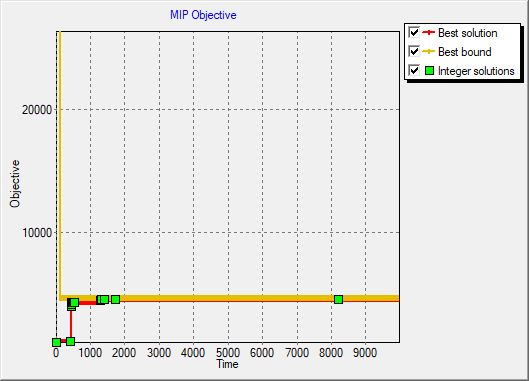
\includegraphics[scale=0.50]{fig/chapter_7/solution_found_edit_zoom_1.png}
    \caption{Graph of when the solutions are found in Mosel Xpress-MP.}
    \label{fig:solutions_found_realized_points}
\end{figure}

In Table \ref{tab:realized_points_diff_gameweeks} one can observe that the optimal solution for 35 gameweeks was not found within maximum running time. As the solution found only has a gap of 0.75 \%, it is regarded as sufficient to serve as a benchmark and compare against the top manager. It is important to note that the objective value given in Table \ref{tab:realized_points_diff_gameweeks} is from the model run, and hence not directly transferable to total points obtained in FPL. To test the model's scalability, the model was run for different number of gameweeks. The results are summarized in Table \ref{tab:realized_points_diff_gameweeks}, and illustrated in Figure \ref{fig:comp_time_diff_gameweeks}. It is notable that the solution time increases significantly when solved for more than 20 gameweeks. %Next, the results from realized points will be discussed into more depth.


\begin{table}[H]
\centering
\resizebox{\columnwidth}{!}{%
\begin{tabular}{@{}llllllll@{}}
\toprule
Number of gameweeks                 & 5       & 10       & 15       & 20       & 25       & 30       & 35      \\ \midrule
%Rows, without presolve    & 24 043   & 48 708    & 73 373    & 98 038    & 122 704   & 147 369   & 172 034 \\
%Rows, presolve            & 22 787   & 47 448    & 72 108    & 96 768    & 121 429   & 146 090   & 170 750 \\
%Columns, without presolve & 35 275   & 71 800    & 108 325   & 144 850   & 181 375   & 217 900   & 254 425 \\
%Columns,, presolve        & 28 124   & 58 045    & 87 962    & 117 897   & 147 778   & 177 640   & 206 689 \\
Objective value           & 773.44 & 1380.95 & 2002.69 & 2660.42 & 3327.12 & 3956.76 & 4553.03 \\
Gap                       & -       & -        & -        & -        & -        & 0.27 \%  & 0.75 \% \\
Time to optimality        & 29      & 295      & 1 103     & 2 010     & 23 692    & N/A      & N/A     \\ \bottomrule
\end{tabular}%
}
\caption{Model run with different number of gameweeks.}
\label{tab:realized_points_diff_gameweeks}
\end{table}

\begin{figure}[H]
    \centering
    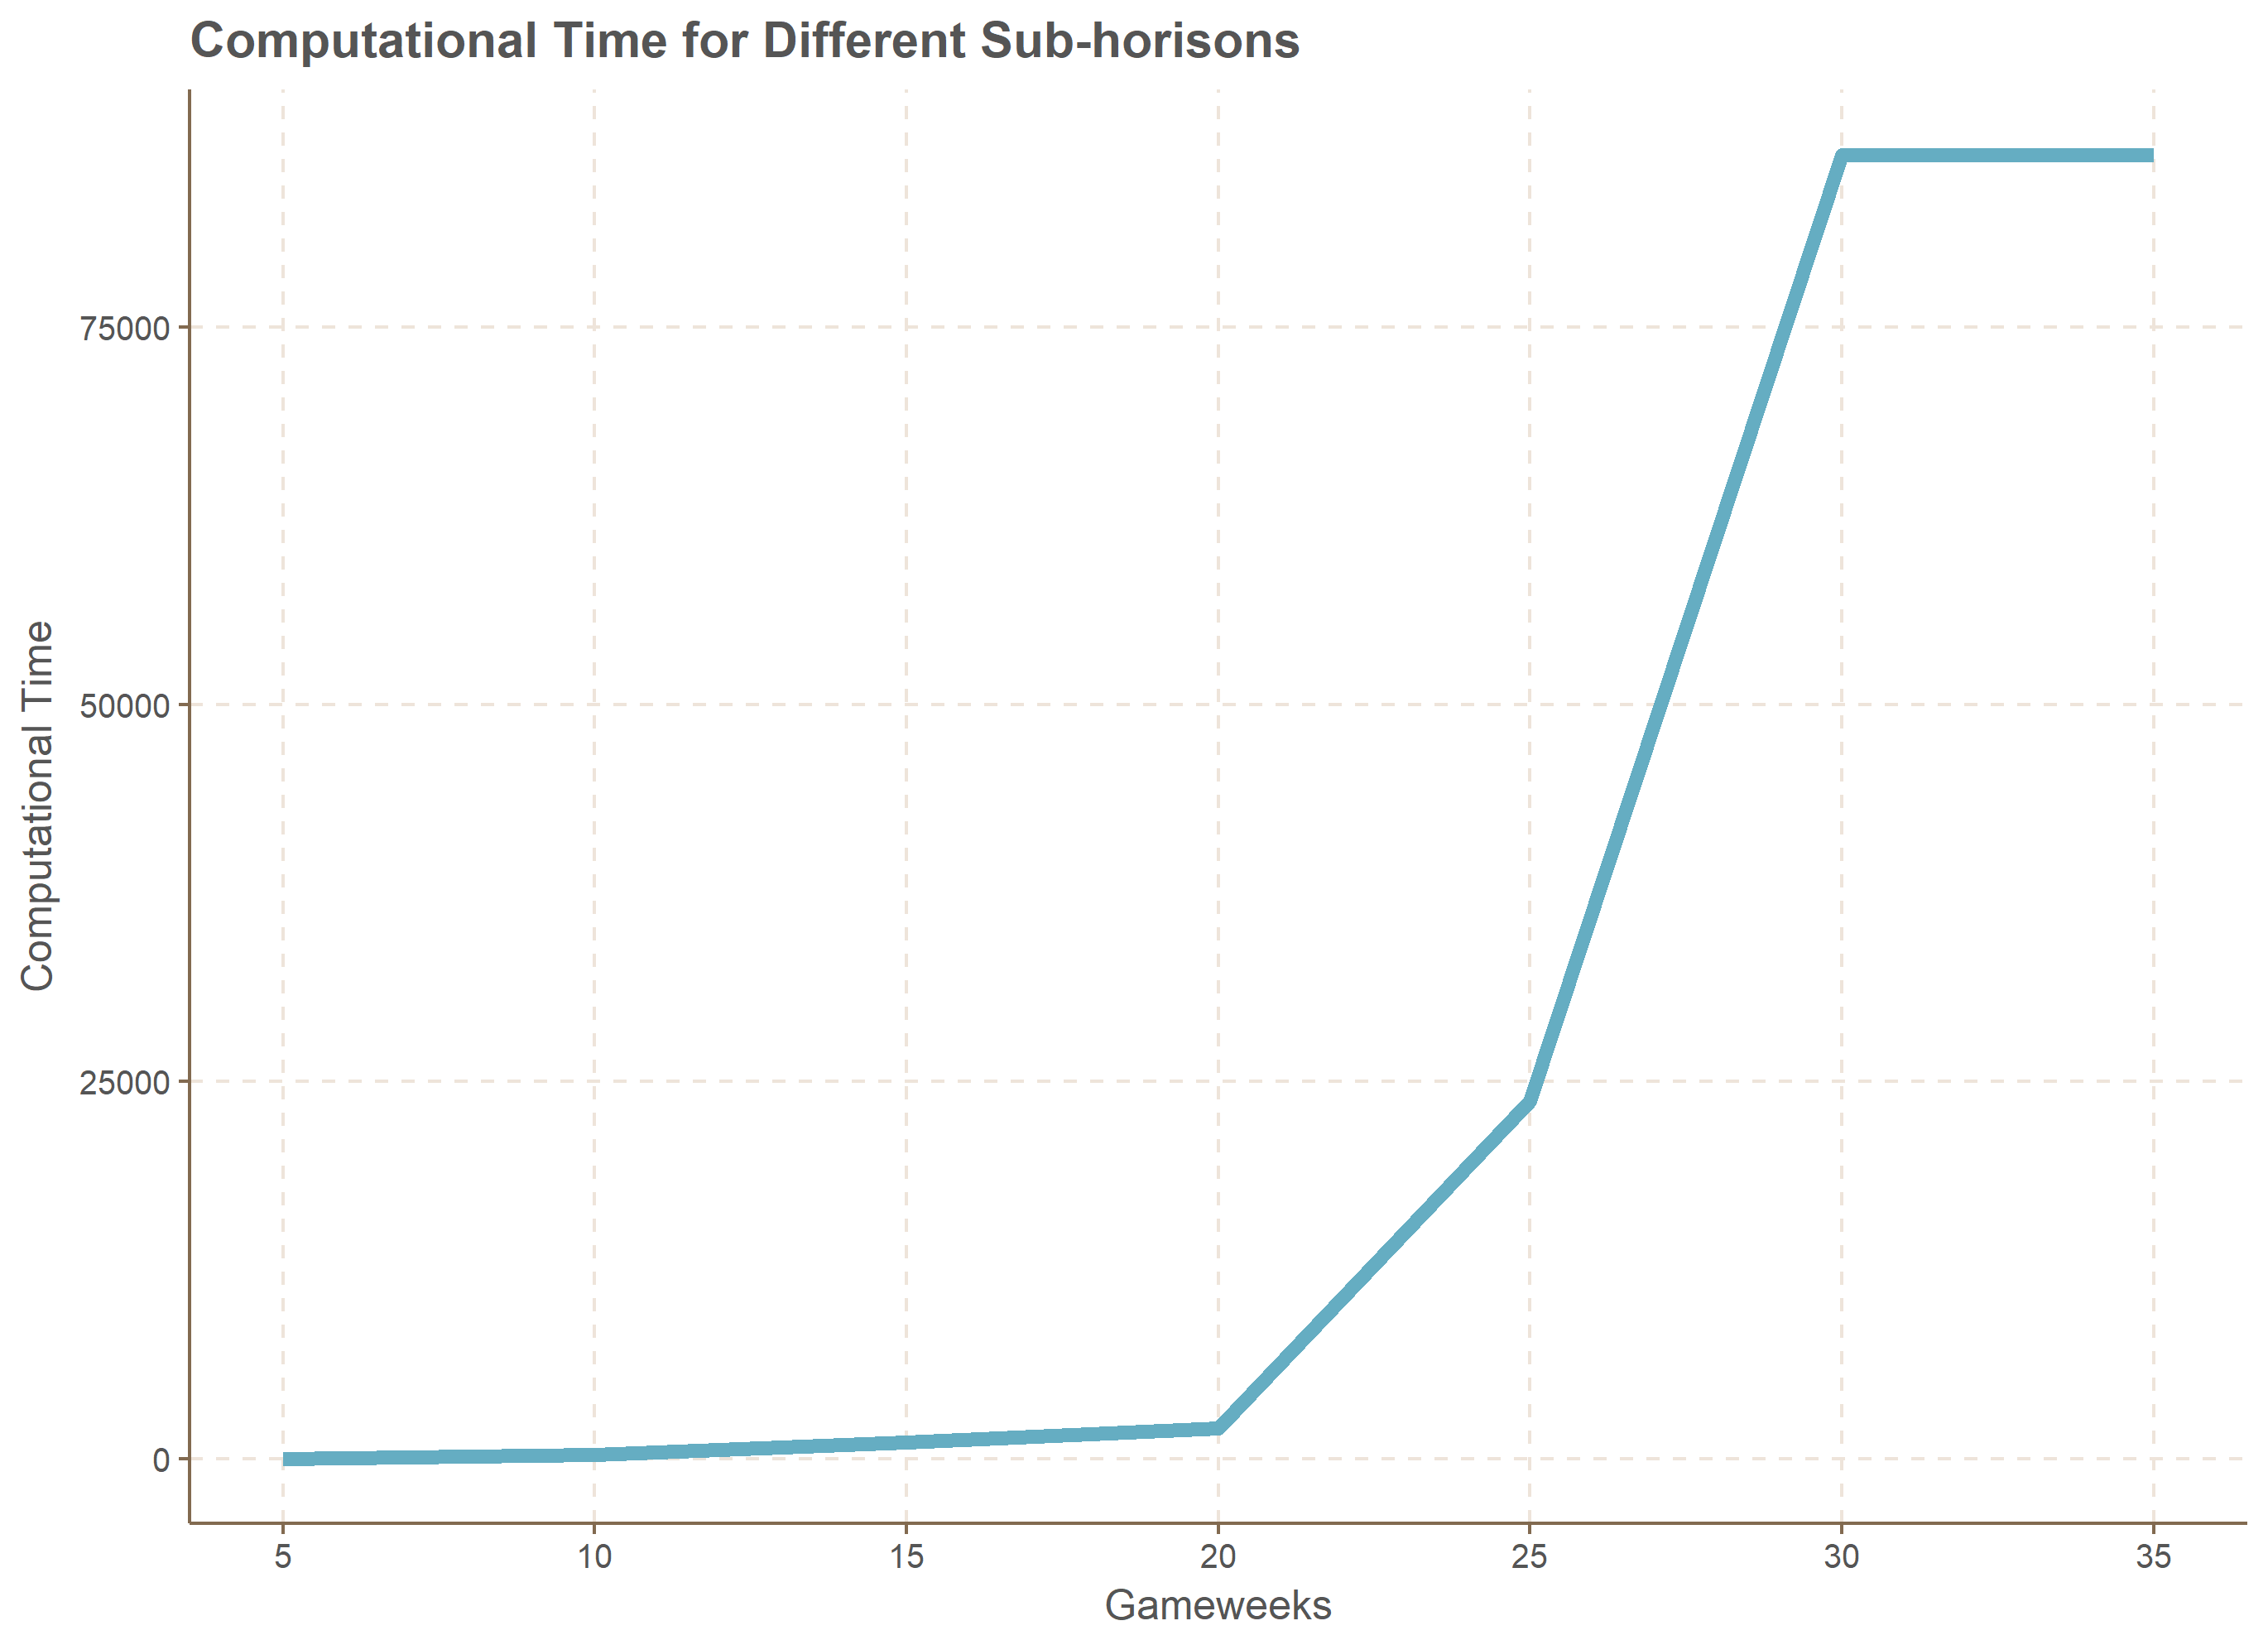
\includegraphics[scale=0.3]{fig/chapter_7/comp_time.png}
    \caption{Plot of solution time when model is solved for different number of gameweeks.}
    \label{fig:comp_time_diff_gameweeks}   
\end{figure}




\subsection{Performance in Fantasy Premier League}
In the following, the performance of the model introduced in chapter \ref{chapter_model_formulation} when solved with realized points, i.e. with perfect information, is presented. Figure \ref{Figure_Realized_points} gives an overview of how many points the model obtained in each gameweek. The coloured dots represents gameweeks where the different gamechips were used. 

\begin{figure}[H]
    \centering
    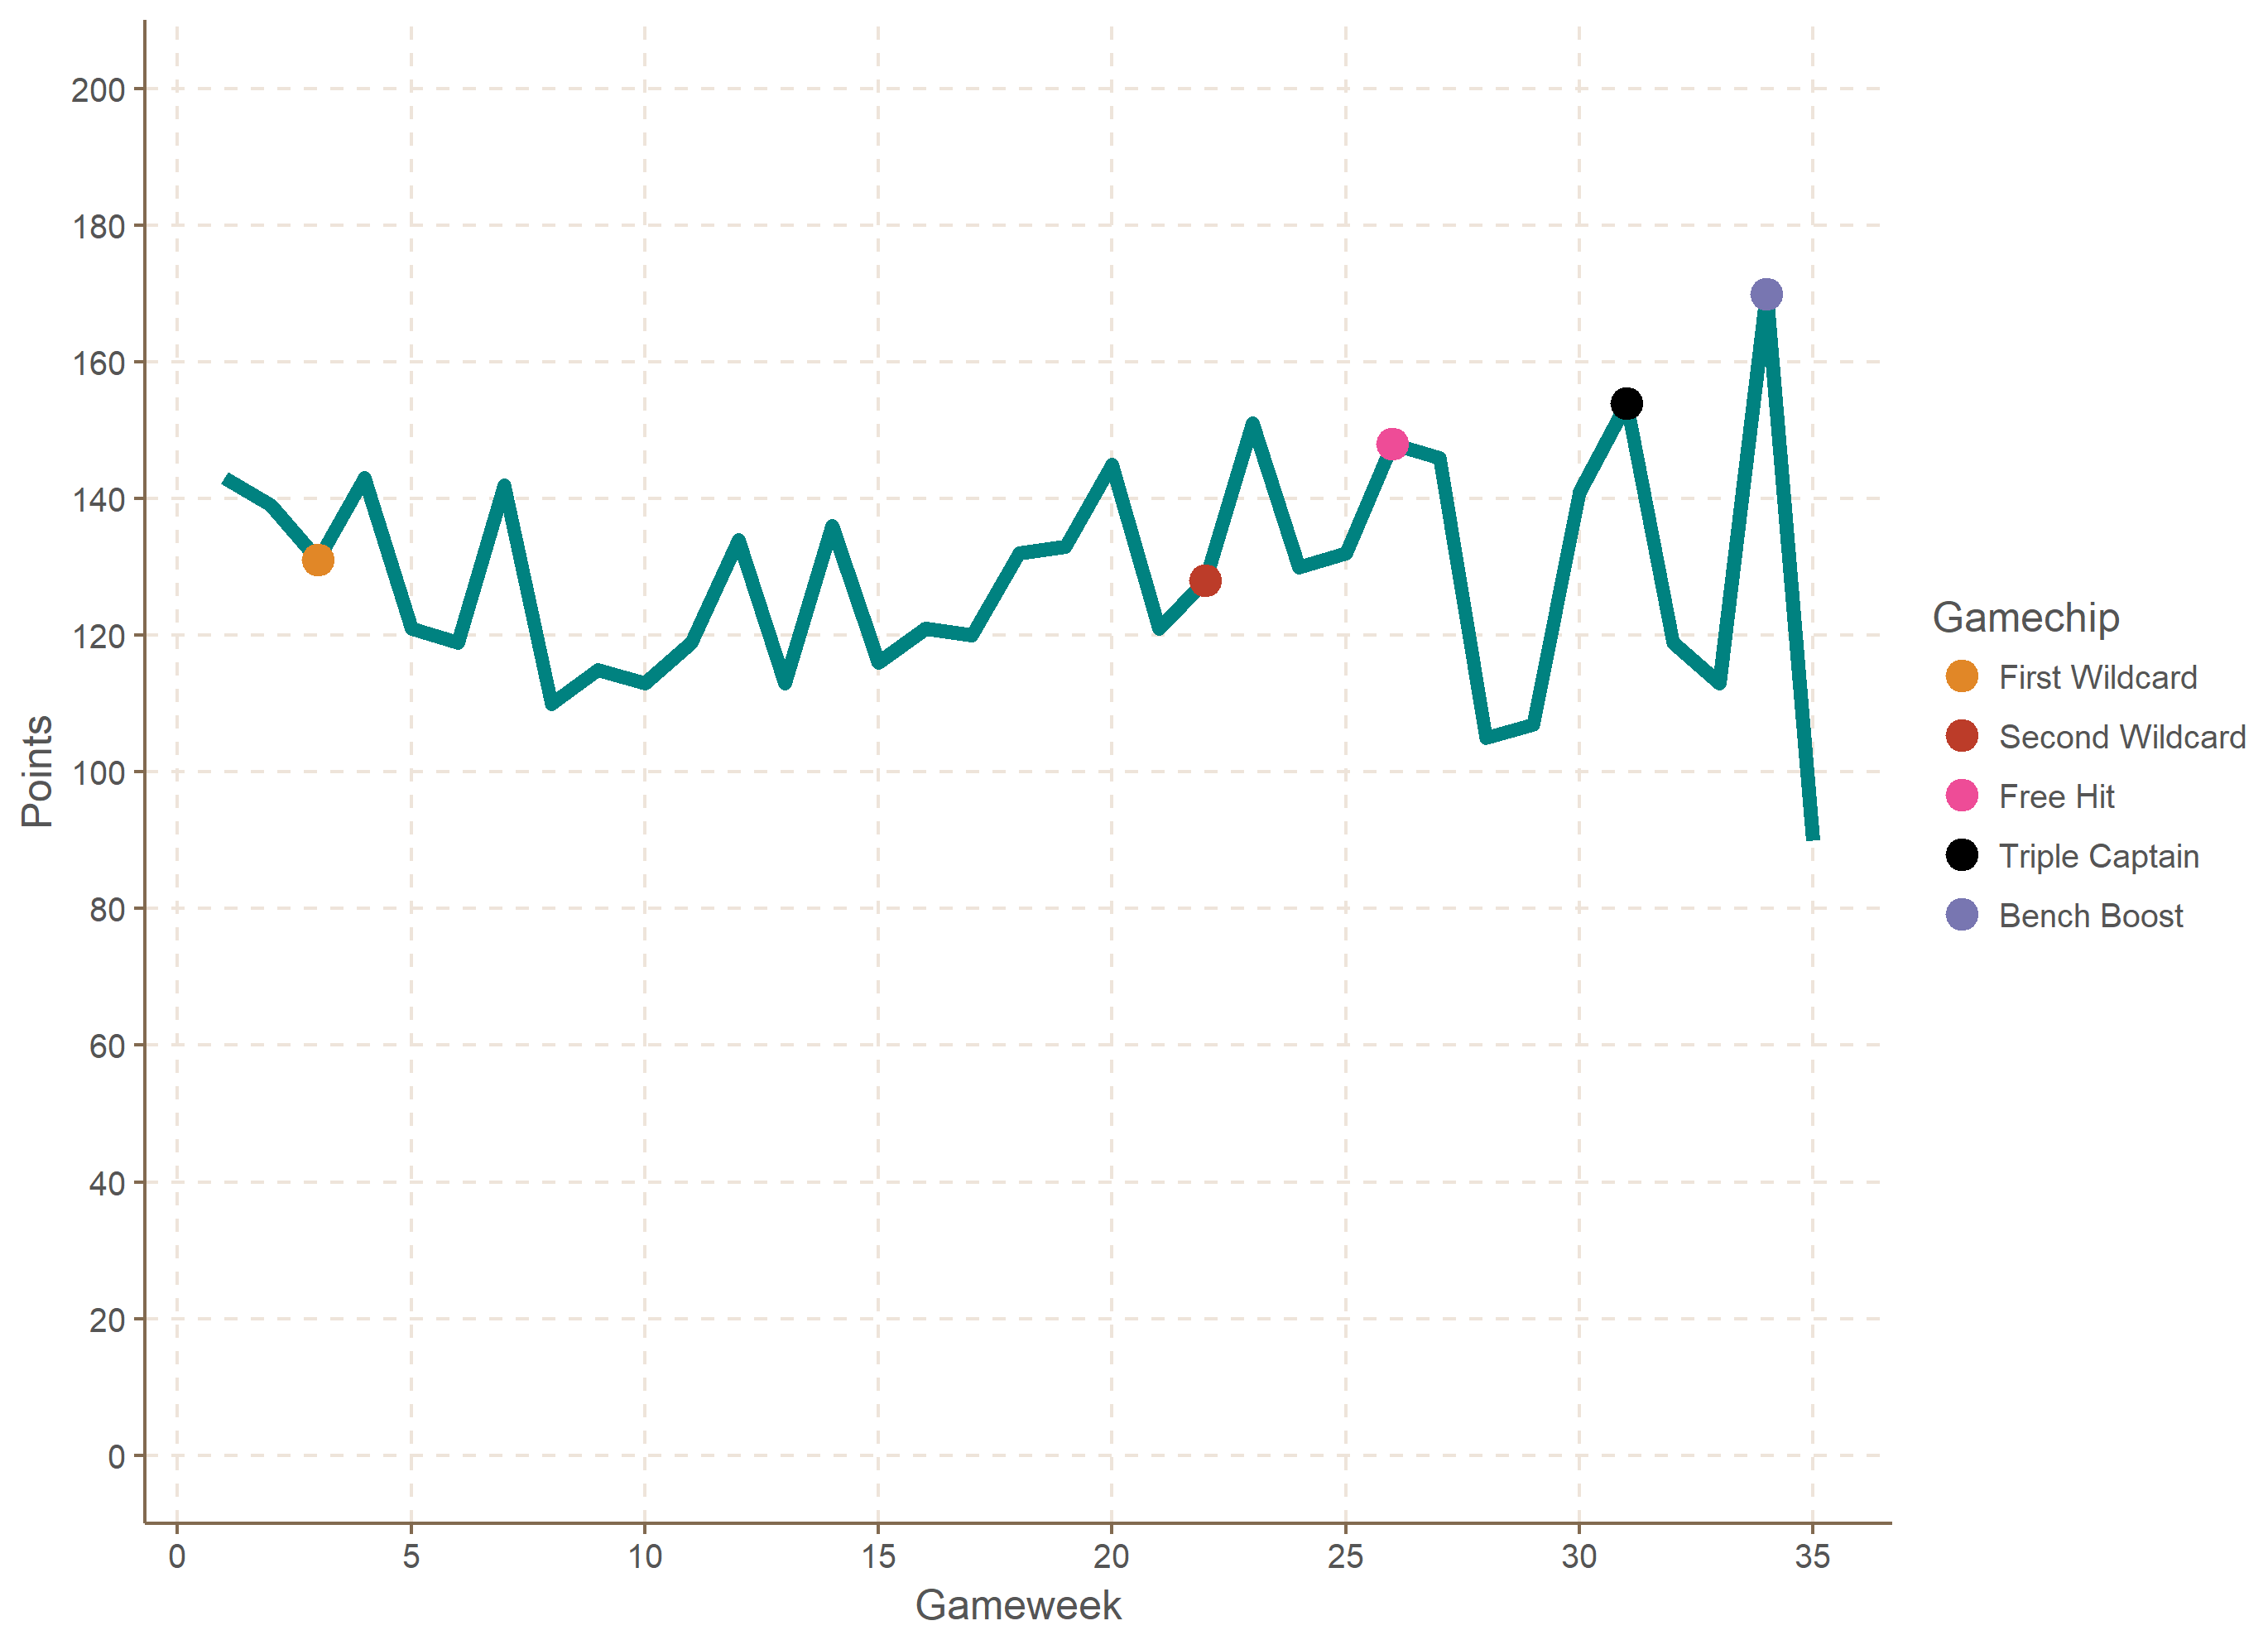
\includegraphics[scale=0.5]{fig/chapter_7/perf_gc.png}
    \caption{The graph shows the points per gameweek with perfect information}
\label{Figure_Realized_points}    
\end{figure}

\begin{comment}
We find it necessary to comment on the choices made for selecting when to play the gamechips.
\end{comment}

As observed from Figure \ref{Figure_Realized_points} both Wildcards were used at early stages after it was allowed to play them. Further, the Triple Captain was played in gameweek 31, which is reasonable as Mohammed Salah scored 4 goals and had 1 assist in this particular gameweek, yielding a score of 29 points. This was the highest score obtained in one gameweek by any Premier League players. The Free Hit was played in gameweek 26, a "normal" gameweek, while the Bench Boost was played in gameweek 34, a double gameweek. Thus, the only gamechip that was used in a way consistent with the implementation in the forecast based optimization model was the Bench Boost. 

\begin{comment}
As observed, the first Wildcard was used one week ahead of the Bench Boost was played. This is reasonable as it is wisely to ensure that you select 15 players that will earn lots of points when playing the Bench Boost. Further, the Free Hit chip was used in gameweek 21, which was a blank gameweek containing only 9 fixtures. It is reasonable to assume that the Free Hit should either be used ahead of a blank or ahead of a double gameweek in order to ensure that all your selected players are featured at least once for that particular gameweek. Finally, the  As for the second Wildcard, there is no obvious reason why it was played in gameweek 26, except the fact that it was optimal for the entire solution. 
\end{comment}


\begin{comment}
Figure \ref{Figure_Transfers} shows how many transfers the model made ahead of each gameweek. It is notable that the model performs most transfers when the Wildcards and the Free Hit were played. This makes sense as these chips allows you to perform unlimited free transfers. In general, one can say that the model makes many transfers compared to human managers. However, this is due to the fact that this is an optimal solution. Thus, it selects the players that over-performed in a particular gameweek. Every gameweek there are some players that surprise the FPL managers. For instance, if a defender suddenly scores two goals in a match, the goals themselves yield 12 points. 

\begin{figure}[H]
\label{fig_Transfers}
    \centering
    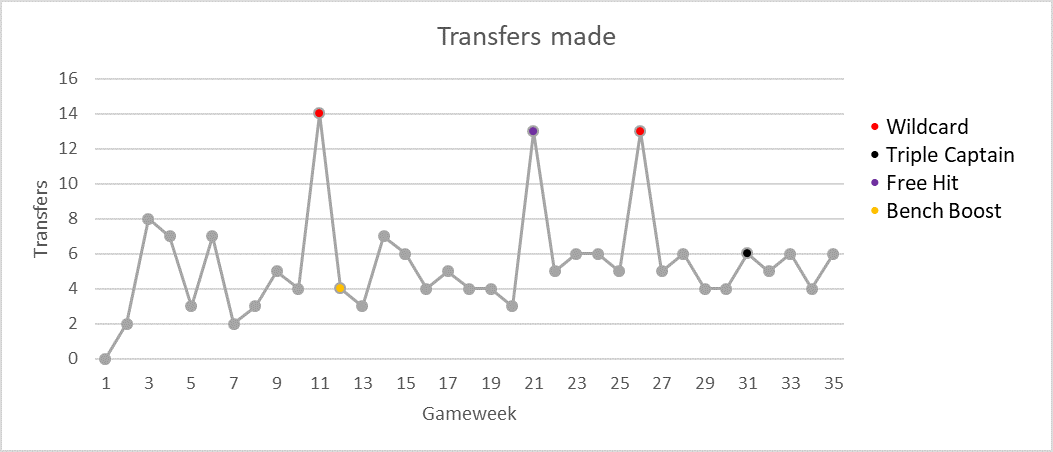
\includegraphics[scale=0.75]{fig/chapter_7/Transfers_colour.png}
    \caption{The graph shows how many transfers the optimal solution makes in every gameweek}
\label{Figure_Transfers}    
\end{figure}

\end{comment}



In Figure \ref{Figure_Comparison} a comparison of the weekly average score among all managers, the score obtained by the top manager and the optimal solution is compared gameweek for gameweek.

\begin{figure}[H]
\label{fig:Comparison}
    \centering
    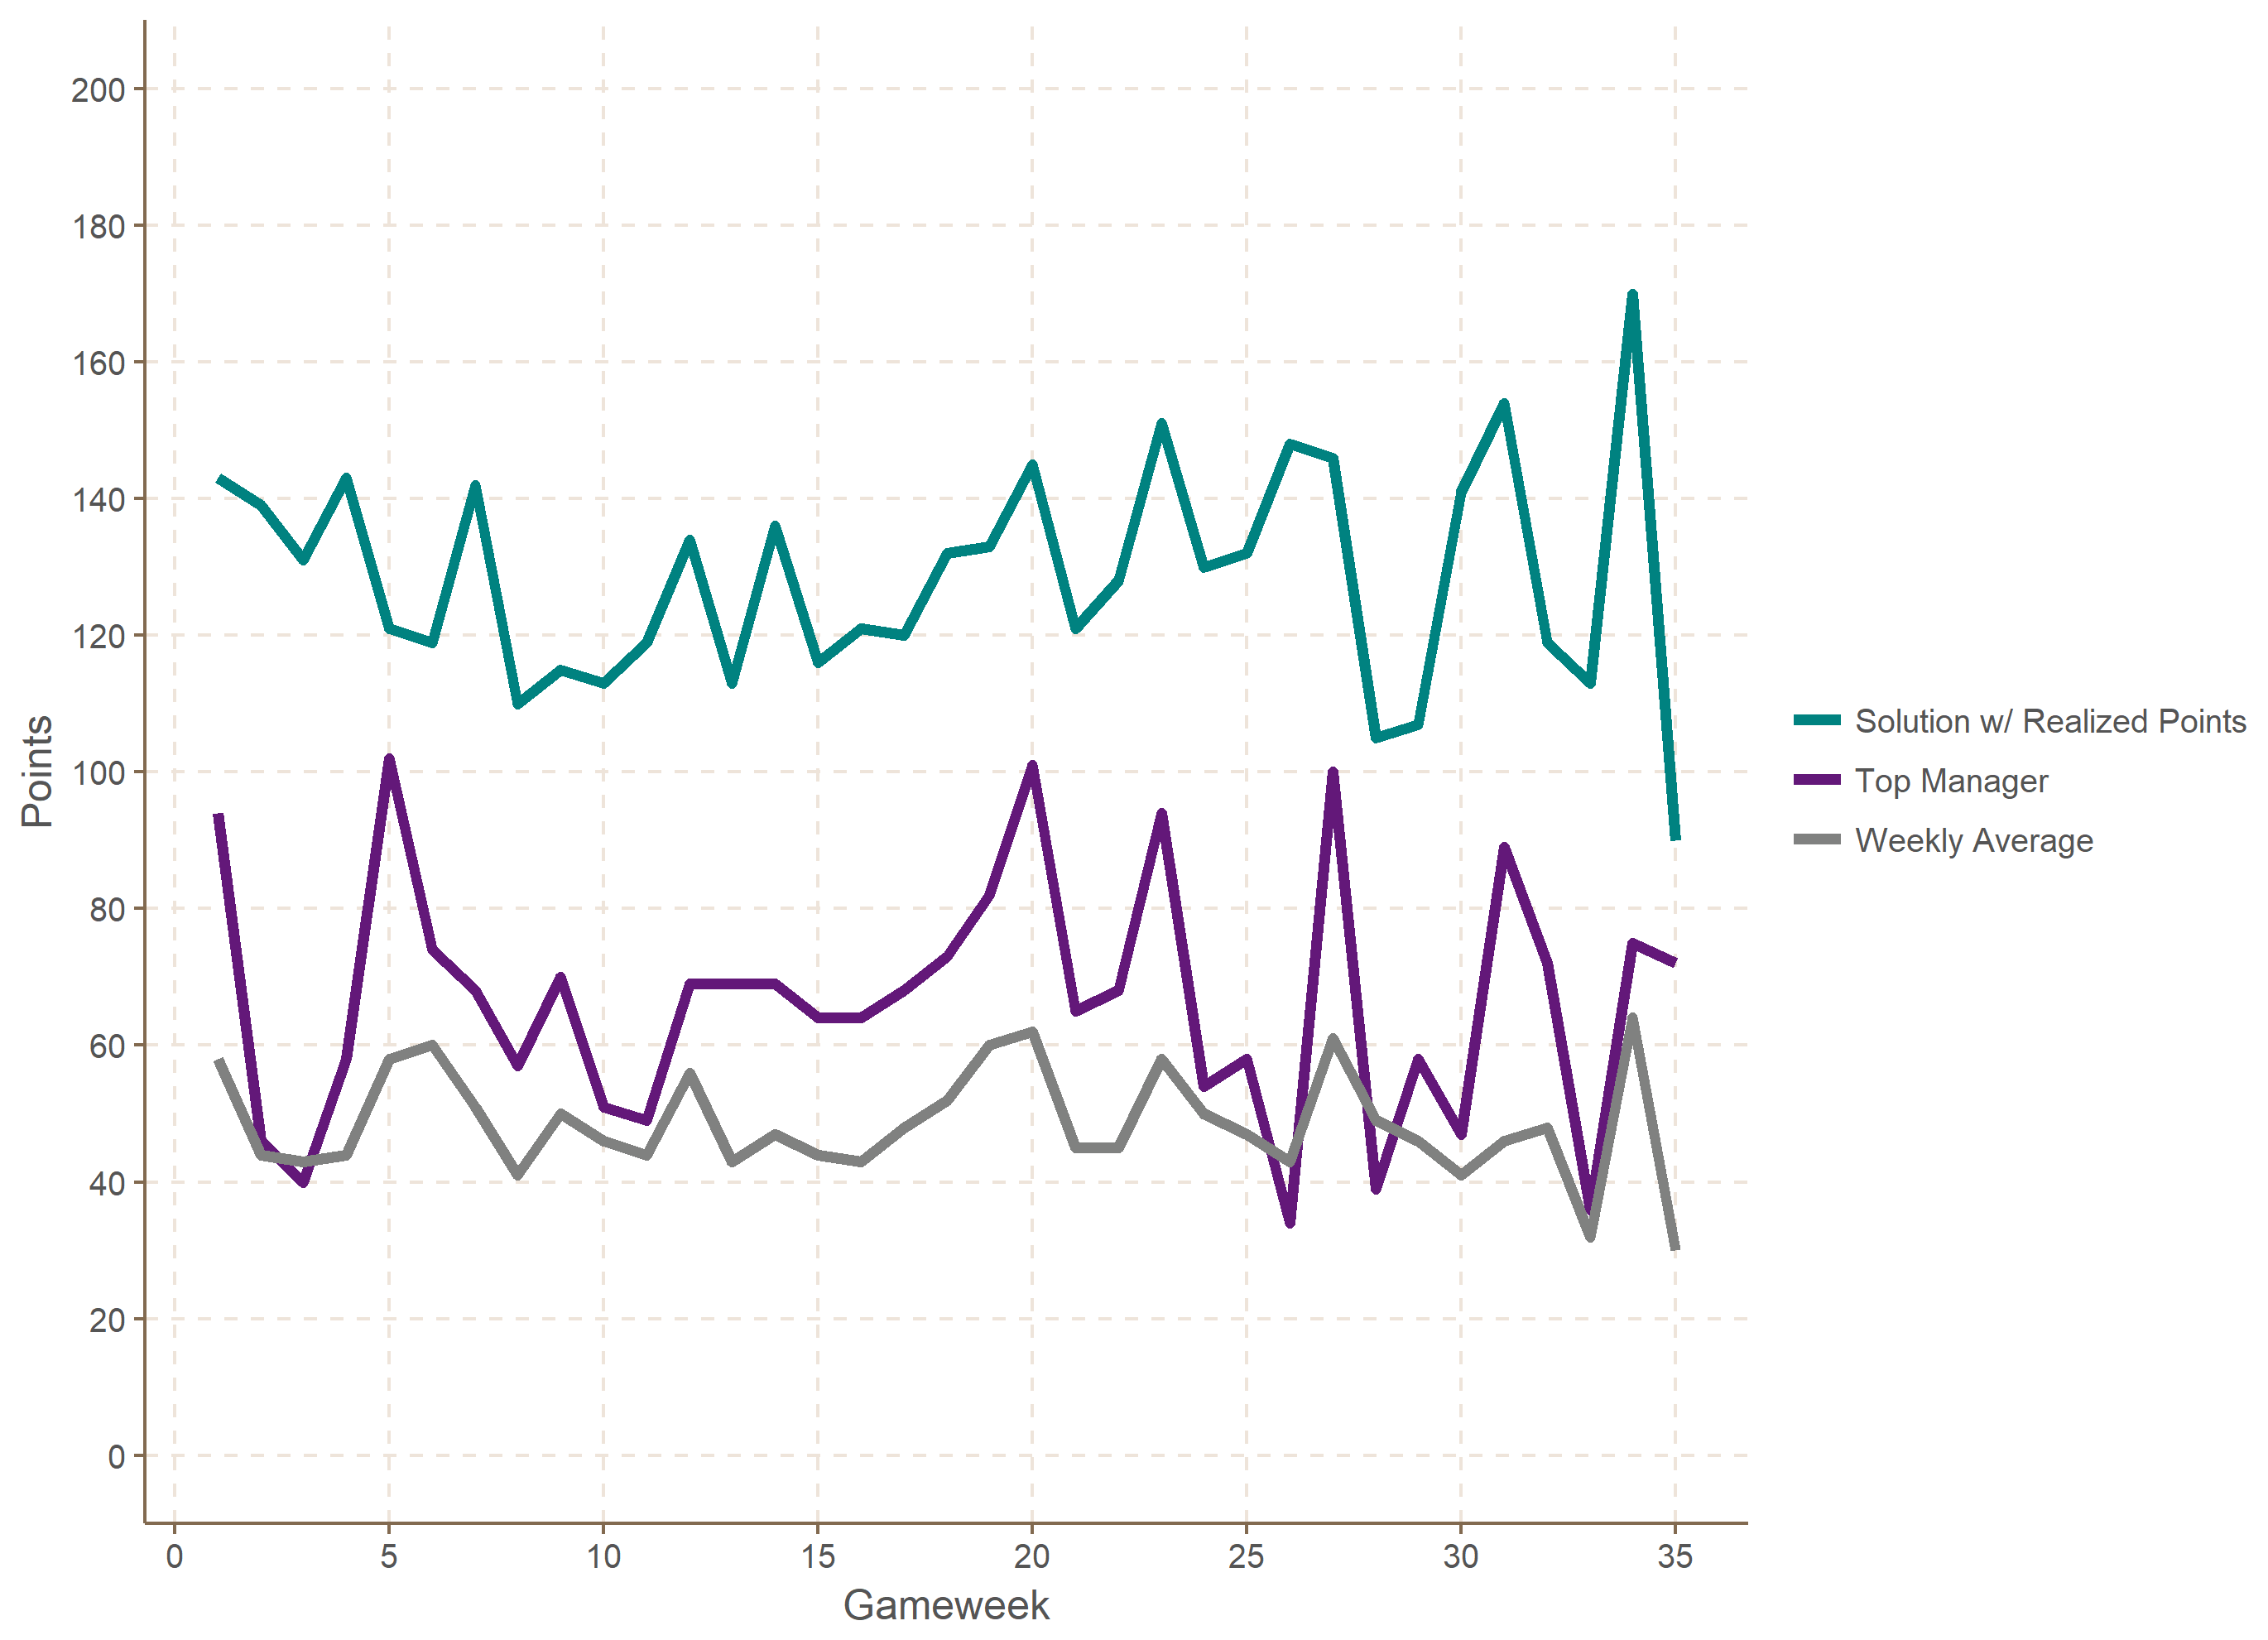
\includegraphics[scale=0.5]{fig/chapter_7/perf_top_avg.png}
    \caption{The graph compares the weekly average and the top performer of each Gameweek to the optimal team with perfect information}
\label{Figure_Comparison}    
\end{figure}

 
From Figure \ref{Figure_Comparison} it is clear that the optimal solution substantially out-performs both weekly average managers, and the top manager in each gameweek. In Table \ref{Optimal_Human} the performance of the top manager as well as the performnce required to reach different rankings among all manager are compared against the optimal solution. It is clear that even the top manager only manages to achieve approximately 50\% of the points obtained by the optimal solution. One implication is that it is extremely hard to compete optimally in FPL, given the nature of the uncertainty of the problem. Moreover, the result can motivate the use of optimization based tools, as there appears to exist a space for improvement.

\begin{table}[H]
\centering
\caption{Comparing human managers to optimal solution}
\label{Optimal_Human}
\begin{tabular}{llc}
\hline
                 & Mean   & \multicolumn{1}{l}{Percentage of optimal solution} \\
\hline                 
Optimal solution & 133.63 & 100.00 \%                                          \\
Top Manager           & 66.54  & 49.80 \%                                           \\
Top 5 \%         & 55.83  & 41.78 \%                                           \\
Top 10 \%        & 54.30  & 40.64 \%                                           \\
Top 20 \%        & 52.20  & 39.06 \%                                           \\
Top 30 \%        & 50.40  & 37.72 \%                                           \\
Top 40 \%        & 48.50  & 36.29 \%                                           \\
Top 50 \%        & 46.50  & 34.80 \%                                           \\
\hline
\end{tabular}
\end{table}

\newpar





\begin{figure}[H]
\label{fig:Top_Manager}
    \centering
    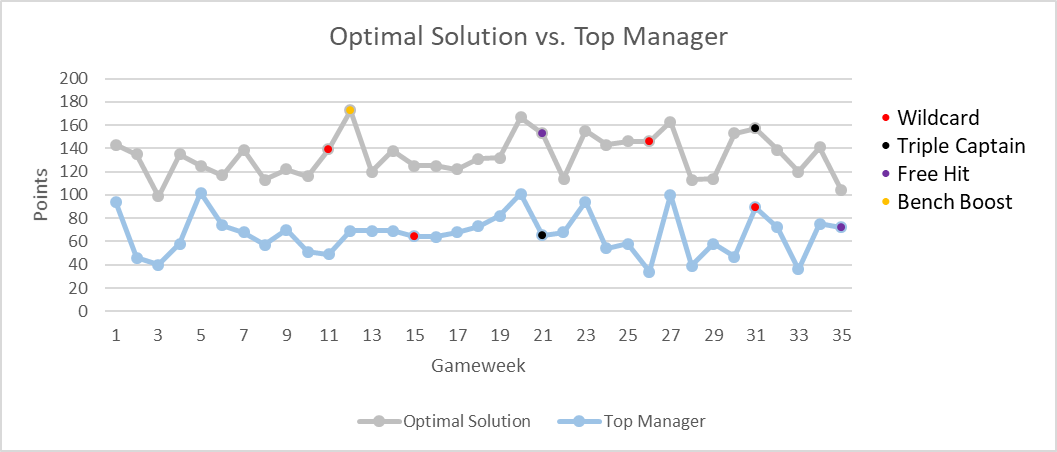
\includegraphics[scale=0.75]{fig/chapter_7/Optimal_vs_Top_colour.png}
    \caption{Comparing optimal solution strategy to top manger}
\label{Top_Manager}    
\end{figure}

As suggested in the introduction, the optimal solution strategy largely outperforms that of the top manager of Fantasy Premier League. In total, it separates 2348 points between the two solutions, more than twice the amount of points gained by the top rated manager. It is notable that the two teams do not play their gamechips in any of the same gameweeks. The top manager played his Triple Captain in gameweek 22, where Tottenham and West Ham were featured twice. Selecting Harry Kane as his Triple Captain is an understandable choice, as Harry Kane was the top scorer of Premier League at that point of time. However, Kane under-performed in both matches only receiving three points in total. In addition, one can see that the top manager played his second Wildcard in gameweek 32, two weeks ahead of a double gameweek. Finally, he played his Free Hit in gameweek 35 which is reasonable as this was ahead of a blank gameweek. As expected, the two teams presented in figure \ref{Top_Manager} are positively correlated.   

\newpar



As observed, it is an enormous difference between the optimal solution strategy and that of the other human managers. It is remarkable that the difference in mean between the top 50\% and the winner is only slightly above 20 points per round, while the difference between the optimal solution and the winner is above 67 points. Further, it is notable that the difference between finishing in the top 10 percentile to the top 5 percentile is rather low as it only separates 1.43 points per gameweek. In comparison, the difference between the winner and the 5th percentile is as much as 10.71 points per gameweek. Moreover, an interesting point is that this difference is actually larger than the one between the 50th percentile and the 5th percentile. Hence, it provides reason to assume that in order to finish among the absolute best managers, one have to perform extremely well compared to others. 
\newpar
 


\section{Forecast-based solutions}\label{sec:inexact}

\begin{comment}
\begin{enumerate}
    \item all the gamechips are explained before this chapter. the implementation of the gamechips do not change in each forecasting method. 
    \item a parameter study on the average method for horizon, penalty and obj.value on average forecasts on season 2016. This has been done before computational study. Suggestion figure: matrix for horizon and penalty, with green = good obj value, red = bad obj value
    \item  the decision on the threshold(risk) is explained in Experimental setup method. 
\end{enumerate}
\end{comment}


In this section, we present the computational results for the three different forecasting methods. First, we present and discuss the performance when gamechips are disregarded. Then, we compare the performance of each method when gamechips are included. Finally, we summarize the results and discuss plausible explanations for the observations made. In order to evaluate the results, we compare the results with the performance of the solution with realized points, the best overall manager and the weekly average among all players. In general, it is important to note that even if no robust statements can be made due to the lack of available data, insightful observations can be made.

\newpage

\subsection{Results Disregarding Gamechips}

In Figure \ref{fig:res_comp_dis_gamechips} the points obtained by the different forecasting methods are plotted for each gameweek. Table \ref{tab:res_dis_gamechips}, summarizes the results. Notice that for the Odds method we have presented results for 31 gameweeks, as we only had data for these gameweeks.

\begin{figure}[H]
    \centering
    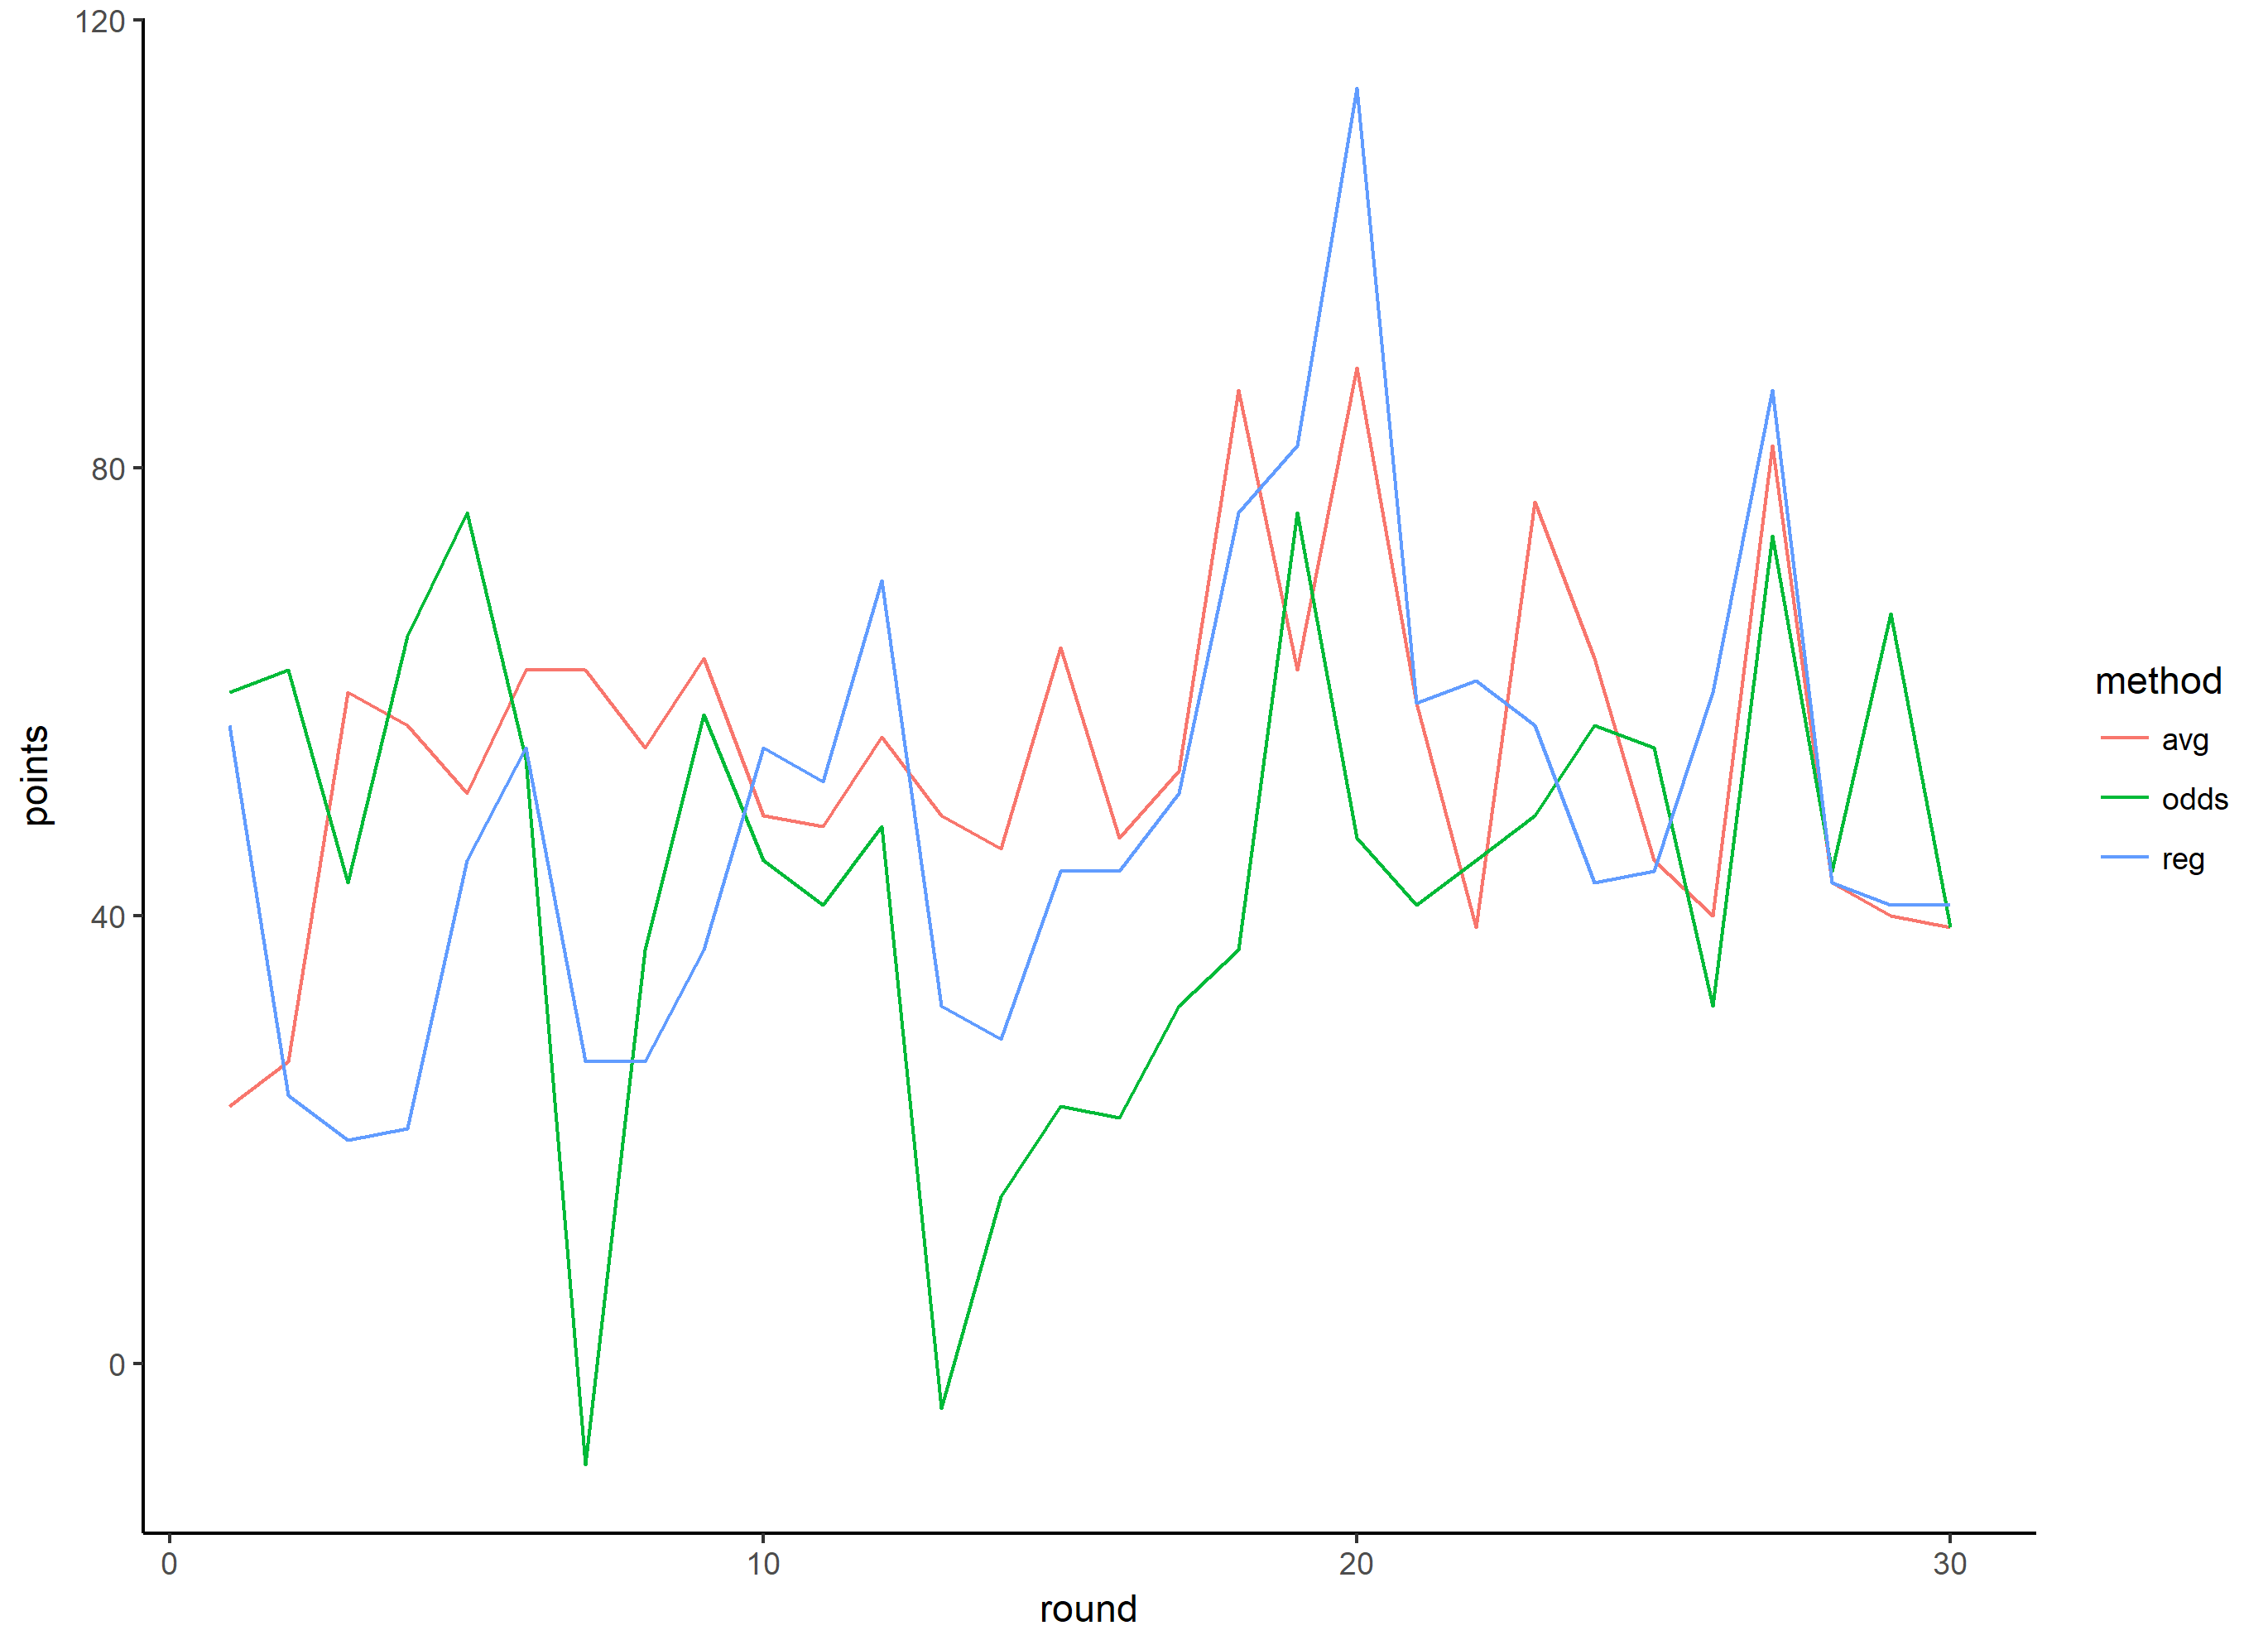
\includegraphics[scale=0.5]{fig/chapter_7/comparison_methods.png}
    \caption{Plot of the results for the different forecasting methods.}
\label{fig:res_comp_dis_gamechips}    
\end{figure}

Comparisons of the overall ranking are made in terms of mean points obtained. This is done because we have considered 31 gameweeks for the Odds method and 35 gameweeks for the two other methods. From Table \ref{tab:res_dis_gamechips}, we see that the Modified Average and the Odds method outperform the Regression method. Moreover, it is clear the mean number of penalized transfers vary considerably between the methods. The difference between the Modified Average and Regression is particularly apparent. 

\begin{table}[H]
\centering
\resizebox{\columnwidth}{!}{%
\begin{tabular}{|l|c|c|c|c|c|}
\hline
Solution method     & Total points & Mean & St.Dev  & Overall ranking & \makecell{Mean penalized \\ transfers}    \\
\hline
Modified Average    & 1916         & 54.74 & 15.85 & Top 8\%   & 0.23       \\
Regression          & 1765         & 50.43 & 20.73 & Top 30\%  & 1.80       \\
Odds (31 gameweeks) & 1650         & 53.23 & 13.94 & Top 13\%  & 0.81       \\
%Odds (28 gameweeks) & 1320         & 47.14 & & Top 47\%  & 0.39       \\
\hline
\end{tabular}%
}
\caption{Results disregarding gamechips.}
\label{tab:res_dis_gamechips}
\end{table}



\begin{comment}
However, from Figure \ref{fig:res_comp_dis_gamechips} it is evident that the Odds method performs better than the two other methods in the first 4 gameweeks. Furthermore, its performance varies significantly during the first half of the season. Note that the odds obtains negative points in gameweek 7 and 13. These were the gameweeks where odds data were missing. As for the Modified Average, its performance increases in the third gameweek. From that point on, the performance stabilizes until gameweek 17, where it increases heavily. Throughout the rest of the season, the Modified Average's performance is greatly improved, reaching scores above 80 points in diverse gameweeks. From Figure \ref{fig:res_comp_dis_gamechips} its observable that the performance of the Regression method is very weak in the first third of the season. However, it tends to increase over the length of the season.
\end{comment}
 

\subsubsection{Modified Average}
\begin{comment}
The Modified Average reaches a total score of 1916 points in the first 35 gameweeks, yielding a mean of 54.74 points per gameweek. In terms of the overall FPL ranking, the Modified Average finishes in the top 8\%.

\newpar
\end{comment}


From Figure \ref{fig:res_comp_dis_gamechips}, it is evident that the Modified Average performs poorly in the first two gameweeks. A reasonable explanation is that the forecasts are based on the previous season. Also, several players are not taken into consideration in the first gameweeks, for instance due to promotions and international transfers. In fact, the Modified Average selects Gary Cahill and Cesc Fabregas, who both received a red card, in the first gameweek. With Cahill selected as captain, they deducted a total of -7 points.

\newpar

It is observable that the weekly results tend to stabilize from gameweek 3 to gameweek 18. This can stem from the fact that forecasts now include the realized points from previous gameweeks in the 2017/2018 season. Hence, the forecasting method is able to select the players who had a good start to the season. In addition, the transferred players from outside Premier League, including players from newly promoted teams, are now assigned expected points.

\newpar

From gameweek 19 to gameweek 35, the Modified Average improves its performance compared to that in the first part of the season. Again, a plausible explanation is that the forecasts are better, by for instance being able to capture which players are performing consistently well.


\subsubsection{Regression}

\begin{comment}
The Regression method reaches a total score of 1765 points in the first 35 gameweeks, yielding a mean of 50.43 points per gameweek. In terms of the overall FPL ranking, the Regression method finishes in the top 30\%.

\newpar
\end{comment}


The Regression method displays a higher variance than the other methods, and reaches the highest weekly realization. However, the method is outperformed by the two other in terms of mean. The weakest weekly performances are obtained in the beginning of the season. This is perhaps explained by the fact the each player is listed with low values for variables such as goals, assists, saves etc, making it hard to distinguish the players from each other. Also, data for the newly promoted teams are scarce, thus limiting possibilities. The method achieves its highest weekly score in gameweek 20, earning 114 points. By comparison, the best overall manager earned 156 points, but played the Triple Captain. Adjusting for the gamechip use, the best manager earned 137 points, leaving a difference of 23 points.

\subsubsection{Odds}
\begin{comment}
The Odds method reaches a total score of 1331 points for 30 gameweeks, and 1320 for 28 gameweeks, yielding a mean of 44.37 and 47.14 points per gameweek, respectively. In terms of the overall FPL ranking, the Odds method finishes in the top 47\% when 28 gameweeks are considered.
\end{comment}


\newpar

The Odds method outperforms the other methods in the first gameweek and has the lowest variance. One explanation is that the forecasts of points are solely based on bookmakers predictions. Since bookmakers are professional, it is not expected that their forecasts will improve greatly over the season. Of course, bookmakers will adjust their calculations based on recent performance of players and teams. However, these adjustment will not be as critical as the adjustments for the two other solution methods. 

\newpar

The Odds method is beaten by the Modified Average method. Although, this does not necessarily mean that bookmakers are poor at setting odds. Remember that bookmakers are profit-seekers, and that the odds they set does not necessarily transfer into real probabilities, but needs to be  lower if bookmakers are to profit from them. Also, the method has a disadvantage in that the data limits us to make forecasts only for one gameweek ahead. That is, the sub-horizon must be equal one.

\begin{comment}

\subsubsection{Discussion}

The Odds method performs best over the first five gameweeks. As mentioned, the Odds method is based on bookmakers odds, and is not as heavily influenced by past season's performance as in the Modified Average and Regression method. In fact, from the previous season's Dream team, i.e. the 11 players that collected most points, only one player had a score above two points in the first gameweek. In addition, the Odds method does not exclude players due to promotion or transfers to Premier League ahead of the season. Furthermore, the Modified Average method outperforms the other methods from gameweek 5-10. One possible reason is that now, the whole track-length is founded in the 2017/2018 season.

\newpar

It appears as if the Regression method is more varying in its performance than the two other methods. This is also evident from the standard deviation presented in Table \ref{tab:res_dis_gamechips}. One explanation is that the Regression method does not account for recent performance in as a direct manner as the Modified Average method does by averaging points in the last rounds. Moreover, the low standard deviation of the Odds method is that the odds are set by the standard procedures of professional bookmakers, while the other methods are solely based on data and will to a larger degree incorporate extreme and unexpected past events.

\newpar

As evident from Table \ref{tab:res_dis_gamechips}, the number penalized transfers is quite different between the methods. In particular, it is high for the Regression method. In fact, it can be argued that the higher penalty term incorporated for Modified Average is only a compensation for inaccurate forecasts. Thus, it appears as if the Regression method in particular could also benefit from a parameter-tuning approach with respect to penalized transfers. However, this was constrained by the lack of data. Hence, it is arguable that it is unfair to compare the performance of the Regression method with the Modified Average method.

\newpar

Without the gamechips, it appears as if it is achievable to reach top 10\%-15\% in terms of overall ranking with our forecasting-based optimization model for the FPL.

\end{comment}






\begin{comment}
Additionally, football is a sport with high uncertainty. Player performances are hard to predict, as factors such as opponents, home field advantage and after all luck affects the performances. 
\end{comment}


\subsubsection{Comparing Modified Average with the solution suggested by \cite{Bonomo}}




We remind reader that the Modified Average method is inspired by the solution approach suggested for the Argentinian Fantasy Football by \cite{Bonomo}. Therefore, we find it interesting to compare the performance of the two different methods. From Figure \ref{fig:avg_vs_bon} and Table \ref{tab:bonomo_mofidified_average}, it is clear that the Modified Average outperforms the approach suggested by \cite{Bonomo}.\cite{Bonomo} set the track-length to 3 and the sub-horizon to 1. Note, however, that the Argentinian fantasy league does not penalize transfers. Therefore, the penalty term is set to 4 as this is stated by the game rules of FPL. Thus, the basis for comparison is somewhat compromised and one should be careful not to draw too categorical statements about the two methods. Regardless, it is apparent that for the 2017/2018, the Modified Average performs constantly better and is a potential improvement of the method.

\begin{figure}[H]
    \centering
    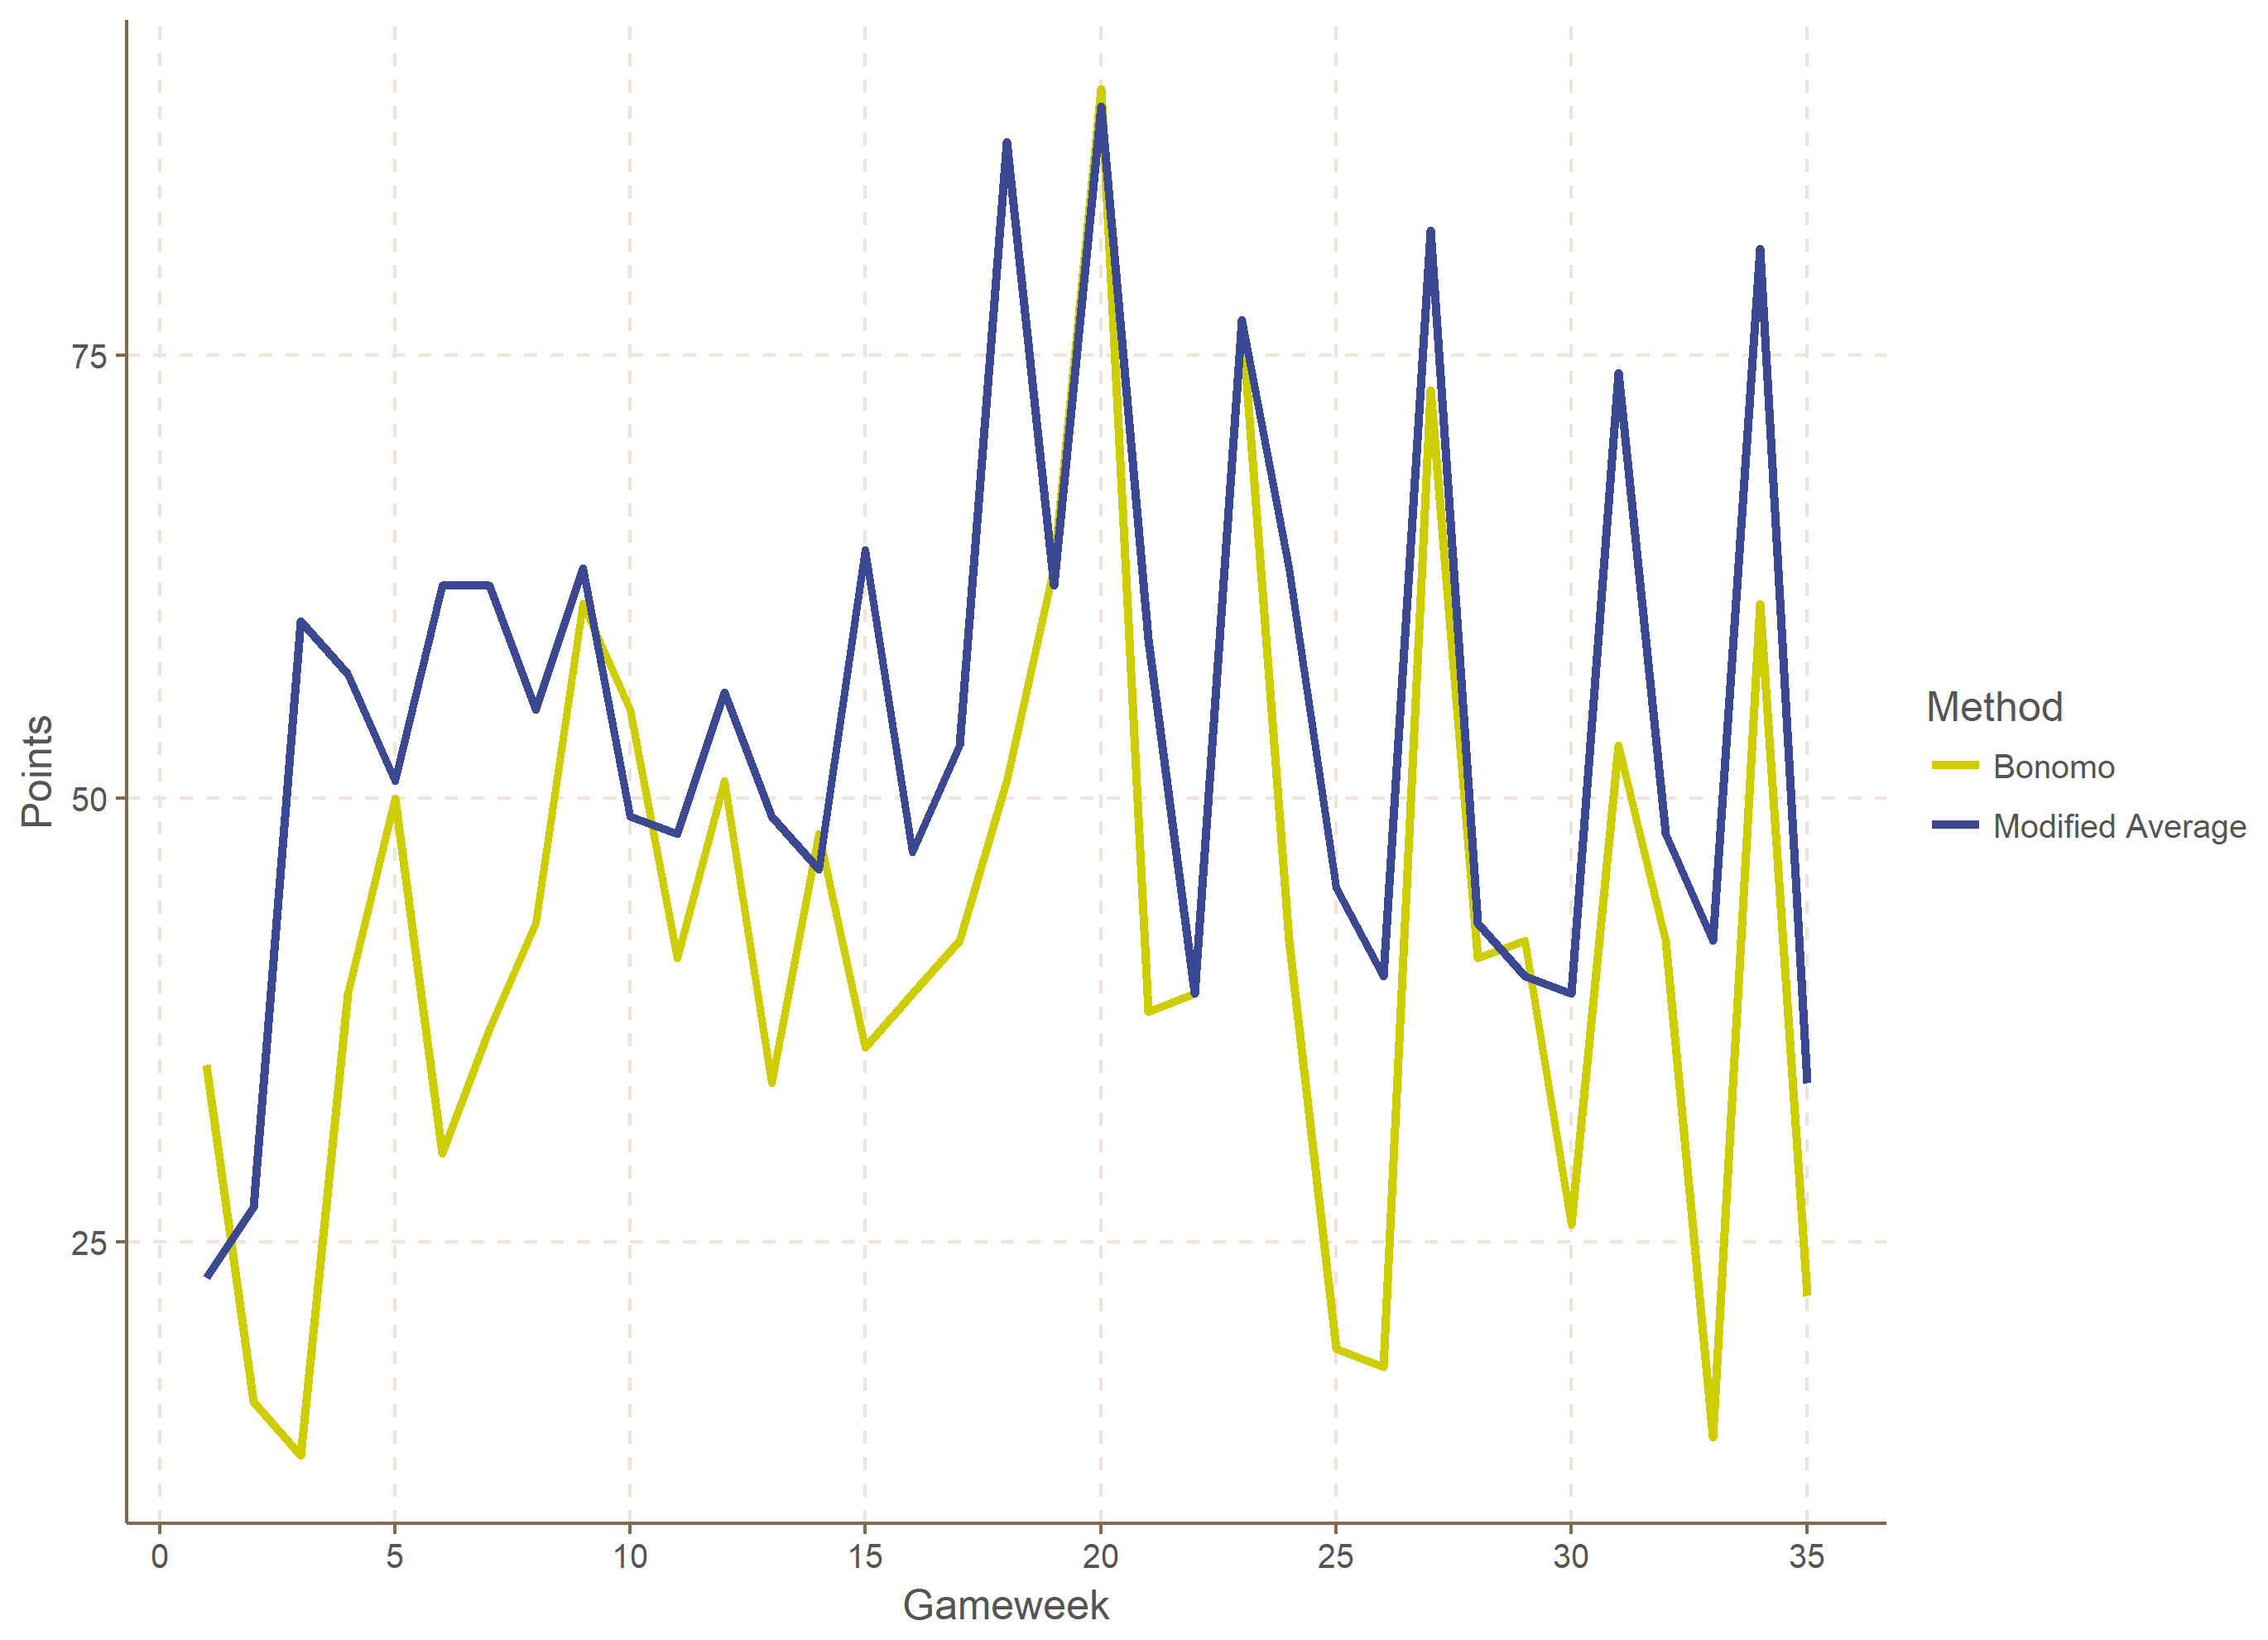
\includegraphics[scale=0.5]{fig/chapter_7/bon_gc_no_gc.png}
    \caption{Comparing performance of Modified Average with the solution approach suggested by \cite{Bonomo}.}
\label{fig:avg_vs_bon}    
\end{figure}

\begin{table}[H]
\centering
\resizebox{\columnwidth}{!}{%
\begin{tabular}{|l|c|c|c|c|c|}
\hline
Solution method     & Total points & Mean & St.Dev  & Overall ranking & \makecell{Mean penalized \\ transfers}     \\
\hline
Modified Average    & 1916         & 54.74 & 15.85 & Top 8\%   & 0.23       \\
\cite{Bonomo}       & 1481         & 42.31 & 17.43 & Top 69\%  & 2.23       \\

\hline
\end{tabular}%
}
\caption{Performance of Modified Average and \cite{Bonomo}}
\label{tab:bonomo_mofidified_average}
\end{table}


\subsection{Results Including Gamechips}

In Table \ref{tab:res_incl_gamechips}, a summary of the performance of each model when including gamechips is presented. Furthermore, the same metrics for the Weekly Average and Top Manager is included for comparison. By comparing the mean obtained with and without gamechips, it is apparent that the effect of gamechips is not consistent for the methods. The Regression method performs better, but both the Modified Average and Odds method perform worse.

\begin{table}[H]
\centering
\resizebox{\columnwidth}{!}{%
\begin{tabular}{|l|c|c|c|c|c|}
\hline
Solution method     & Total points & Mean & Std.Dev  & Overall ranking & \makecell{Mean penalized \\ transfers} \\
\hline
Modified Average    & 1881         & 53.74 & 16.62 & Top 12\%   &  0.23   \\
Regression          & 1901         & 54.31 & 20.32 & Top 10\%   &  1.20   \\
Odds (31 gameweeks) & 1557         & 50.23 & 15.17 & Top 30\%   & 0.48   \\
Weekly Average      & 1699         & 48.53 & - & Top 40\%   &  - \\
Top Manager         & 2329      & 66.54 & 18.02 &  Top 1 ‰   & 0.11\\
\hline
\end{tabular}%
}
\caption{Results including gamechips.}
\label{tab:res_incl_gamechips}
\end{table}



In Figure \ref{fig:res_comp_gamechips}, each method is plotted with and without gamechips. In the following, we discuss how each gamechip have effected the solutions. Note that for each method, points obtained are similar for the first 6 gameweeks. As mentioned in Section \ref{exp_setup_gamechips} the model was allowed to use a Wildcard in gameweek 9, hence this decision was first considered in gameweek 7 due to the sub-horizon of three gameweeks. Therefore, the models make different decisions from that point on.

\begin{figure}[H]
    \centering
    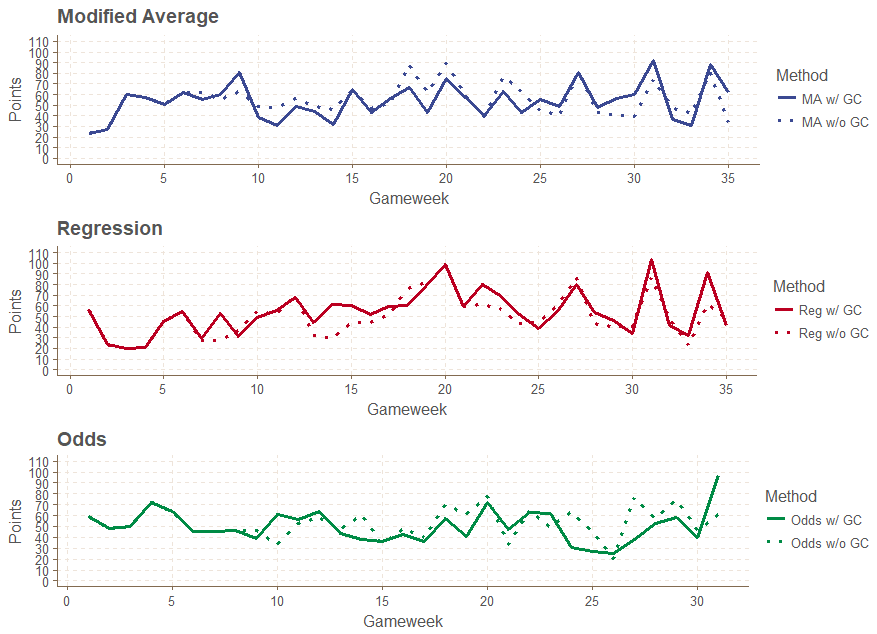
\includegraphics[scale=0.5]{fig/chapter_7/w_wo_gc_all.png}
    \caption{Comparing performance with gamechips.}
\label{fig:res_comp_gamechips}    
\end{figure}


To evaluate the impact of the first Wildcard,  we begin by comparing performances from gameweek 7, as this is the first gameweek were decisions regarding the Wildcard are introduced. Moreover, we only measure the effect until gameweek 19, as decisions regarding the Triple Captain are first introduced in this gameweek. As expected, Table \ref{tab:first_wildcard} shows that all methods perform a substantially higher number of transfers when the Wildcard is played. However, the effect of these transfers appear to be rater limited for the Modified Average and Odds method, as both performs worse in these gameweeks with the Wildcard. The Regression on the other hand, performs considerably better when the Wildcard is used.  

\newpar




\begin{table}[H]
\centering
\begin{tabular}{@{}lcc@{}}
\toprule
                Method  & Mean GW 7-19  & Transfers GW 9 \\ \midrule
Modified Average w/gc   & 51.08 & 11             \\
Modified Average w/o gc & 57    & 1              \\
Regression w/gc         & 53.92 & 12             \\
Regression w/o gc       & 48.15 & 5              \\
Odds w/gc               & 46.62 & 11             \\
Odds w/o gc             & 49.31 & 1              \\ \bottomrule
\end{tabular}
\caption{Performance from gameweek 7 to 19.}
\label{tab:first_wildcard}
\end{table}


As can be seen in Table \ref{tab:performance_triple_captain}, all methods select either Harry Kane or Son Heung-min as Triple Captain in gameweek 22. First, it is worth noting that all players play for Tottenham, one of two teams that had a double gameweek. Furthermore, the Regression and Odds method had both players in their starting line-ups. Thus, both the Regression and Odds had a higher forecast for Son Heung-min than Harry Kane. A curious observation is that it was speculated in whether Kane would play both matches or not. Such events can be caught by the Regression method by the variables number of transfers in and transfers out, and by the odds set by the decisions of bookmakers. For the Modified Average method, however, there is no way to pick up such signals. By not being able to incorporate any qualitative information such as line-up rumours, the Modified Average has a disadvantage when it comes to making the important decision as who to select for Triple Captain.

\begin{table}[H]
\centering
\begin{tabular}{@{}lcc@{}}
\toprule
                 Method       & Triple Captain & Points \\ \midrule
Modified Average w/gc   & Harry Kane           & 9      \\
Modified Average w/o gc & Harry Kane           & 6      \\
Regression w/gc         & Son Heung-min            & 36     \\
Regression w/o gc       & Son Heung-min            & 24     \\
Odds w/gc               & Son Heung-min            & 36     \\
Odds w/o gc             & Son Heung-min            & 24     \\ \bottomrule
\end{tabular}
\caption{Performance of Triple Captain in gameweek 22.}
\label{tab:performance_triple_captain}
\end{table}

\newpar 

From Figure \ref{tab:performance_free_hit}, it is apparent that all methods perform better in the blank gameweek 31 the Free Hit is used with a difference of approximately 20 points. Furthermore, it is notable that only the Odds method makes a substantial amount of transfers ahead of the blank gameweek. This can be explained by the sub-horizon of 1, as the other methods can plan 3 matches ahead. For the Modified Average there are large differences in the number of players playing with and without gamechips, compared to the other methods. 
This can be due to the fact that the parameter tuning was done without taking the Free Hit into consideration. Hence, a penalty term of 16 is perhaps not optimal. It is worth noting that all methods obtain a relatively high score for the gameweek. This is mostly explained by the fact that Mohammed Salah earned 29 points for the particular gameweek. As all methods had him as captain, they earned a score of 58 points on him alone.

\begin{table}[H]
\centering
\begin{tabular}{@{}lccc@{}}
\toprule
Method                  & Points GW31 & Transfers  & Players playing \\ \midrule
Modified Average w/gc   & 92          & 14         & 11              \\
Modified Average w/o gc & 74          & 0  & 5               \\
Regression w/gc         & 104         & 13         & 11              \\
Regression w/o gc       & 87          & 2  & 9               \\
Odds w/gc               & 97          & 15         & 11              \\
Odds w/o gc             & 61          & 10  & 11              \\ \bottomrule
\end{tabular}
\caption{Performance of Free Hit in gameweek 31.}
\label{tab:performance_free_hit}
\end{table}


\newpar

As the second Wildcard and Bench Boost are played in cooperation, they are discussed together. The second Wildcard was played in gameweek 33, preparing for the double gameweek 34. As data for these gameweeks only are available for the Modified Average and Regression method, the discussion is limited to these methods. Since the Bench Boost is played in gameweek 34, it is considered by the model from gameweek 32. Since gameweek 31 is the gameweek when the Free Hit is played, we have considered gameweek 32-34 when evaluating the effect of the second Wildcard and Bench Boost. Table \ref{tab:performance_wildcard_and_bench_boost} shows that in terms of mean points obtained, the effect of the Wildcard and Bench Boost for gameweek 32-34 is positive only for the Regression method. In particular, the Modified Average again performs weaker in the gameweek the Wildcard is played, while the Regression performs better. Furthermore, both methods improves in the gameweek the Bench Boost is played. However, as 15 players are awarded points, this is not unexpected.


\begin{table}[H]
\centering
\begin{tabular}{@{}llccc@{}}
\toprule
Method                  & GW 32 & GW 33 (W) & GW 34 (BB) & Mean \\ \midrule
Modified Average w/gc   & 37    & 31        & 88         & 52   \\
Modified Average w/o gc & 48    & 42        & 81         & 57   \\
Regression w/gc         & 42    & 32        & 91         & 55   \\
Regression w/o gc       & 48    & 23        & 61         & 44   \\ \bottomrule
\end{tabular}
\caption{Performance of Wildcard and Bench Boost in GW32-34.}
\label{tab:performance_wildcard_and_bench_boost}
\end{table}






\subsection{Summary}

\begin{table}[H]
\centering
\resizebox{\columnwidth}{!}{%
\def\arraystretch{1.5}
\begin{tabular}{|l|c|c|c|c|c|}
\hline
Solution method            & Total points              & Mean                       & Std.Dev                    & Overall ranking               & \makecell{Mean penalized \\ transfers} \\ \hline
Modified Average w/ gc     & 1881                      & 53.74                      & 16.62                      & Top 12\%                      & 0.23                                                                                \\ \hline
Modified Average w/o gc    & 1916                      & 54.74                      & 15.85                      & Top 8\%                       & 0.23                                                          \\ \hline
Regression w/ gc           & 1901                      & 54.31                      & 20.32                      & Top 10\%                      & 1.20                                                                                \\ \hline
Regression w/o gc          & 1765                      & 50.43                      & 20.73                      & Top 30\%                      & 1.80                                                           \\ \hline
Odds (31 gameweeks) w/ gc  & 1557                      & 50.23                      & 15.17                      & Top 30\%                      & 0.48                                                                                \\ \hline
Odds (31 gameweeks) w/o gc & 1650                      & 53.23                      & 13.94                      & Top 13\%                      & 0.81                                                           \\ \hline
Realized points            & 4500                         & 128.57                          & 16.50                          & NA                             & 4.23  
                             \\ \hline
Weekly Average             & 1699                      & 48.53                      & 7.99                       & Top 40\%                      & -                                                                                   \\ \hline
Top Manager                & 2329                      & 66.54                      & 18.28                      & Top 1 ‰                       & 0.11                                                                                \\ \hline
\end{tabular}%
}
\caption{Summary of the results.}
\label{tab:summary_of_results}
\end{table}



In Table \ref{tab:summary_of_results}, the results of all different methods with and without gamechips are summarized. Furthermore, the solution with realized points are also given to use as a benchmark. However, the model with realized points significantly beats the forecast-based optimization model. Therefore, as a more realistic benchmark for top performance, the performance of the top manager is included. As a benchmark of average performance, the FPL's weekly average is used.

\newpar

The best manager only manages to achieve ?\% of what the solution with realized points does. This speaks in volumes of the overall uncertainty in the FPL. Furthermore, it motivates the potential of data-driven models. With either the Modified Average forecasting approach, or the Regression based approach with gamechips, our forecast-based optimization model appears to have the potential to reach among the top 10\% of managers in the FPL. However, as we only have tested on one season, overly categorical statements should not be made. Regardless, a position in the top 30\% is achieved by all marks. Thus, beating the average weekly performance certainly appears to be obtainable. As the season consists of 38 gameweeks, comparing overall performance is somewhat biased when we only look at gameweek 1-35. For instance, some managers may still have gamechips left. This is also the case when comparing Odds to the other methods. Nevertheless, the results should be indicative as more than 5.5 million people play the game and plenty will already have played all the gamechips.

\newpar

The Odds method performs best over the first five gameweeks. As the Odds method is based on bookmakers odds, it is not as heavily influenced by past season's performance as the Modified Average and Regression method. In fact, from the previous season's Dream team, i.e. the 11 players that collected most points, only one player had a score above two points in the first gameweek. In addition, the Odds method does not exclude players due to promotion or transfers to Premier League ahead of the season. Furthermore, the Modified Average method outperforms the other methods from gameweek 5-10. One possible reason is that now, the whole track-length is founded in the 2017/2018 season.

\newpar

As evident from Table \ref{tab:summary_of_results}, the number penalized transfers is quite different between the methods. In particular, it is high for the Regression method. In fact, it can be argued that the higher penalty term incorporated for Modified Average is only a compensation for inaccurate forecasts. Thus, it appears as if the Regression method in particular also could benefit from a parameter-tuning approach with respect to penalized transfers. However, this was constrained by the lack of data. Hence, it is arguable that it is unfair to compare the performance of the Regression method with the Modified Average method. Hence, a potential for parameter tuning exists for the Regression method when more data is available, and is an exciting topic for future research.

\newpar 

In general, the methods exhibit different volatility. It appears as if the Regression method is more varying in its performance than the two other methods and the Odds method has lowest variability. This is also evident from the standard deviations presented in Table \ref{tab:summary_of_results}. One explanation is that the Regression method does not account for recent performance in as a direct manner as the Modified Average method does by averaging points in the last rounds. Moreover, odds are set by the standard procedures of professional bookmakers, while the other methods are solely based on data and will to a larger degree incorporate extreme and unexpected past events. Moreover, the performance for all methods appear to fluctuates more in the second half of the season. One sensible reason is the emergence of blank and double gameweeks. 

\newpar

The effect of gamechips is not consistent for all methods. The Triple Captain and Free Hit appears to boost performance for all methods. The Second Wildcard in combination with Bench Boost appear to have a favorable effect on the Regression model, but not for the Modified Average. The same goes for the first Wildcard. This can be due to several reasons. First, for the Regression method in Section \ref{exp_setup_reg}, it is found that time-series effect of points is rather limited. Hence, for the Regression, only variables such as total amount of goals, saves etc are considered. When playing the Wildcard, the entire selected squad can be changed, and the new selected squad is carried forwards. If the Wildcard is played and forecasts are based on the Regression method, the performances of players over all the previous gameweeks are considered. For the Modified Average, on the other hand, the forecasts are only based on the last 5 matches. When considering to change the entire selected squad, i.e. playing the Wildcard, taking the all previous gameweeks into consideration seems to be the preferable approach. Secondly, the parameter tuning is done without gamechips in mind. That is, neither track length nor sub-horizon are optimized with respect to the Wildcard.

It is rather counter intuitive that the results are worse when including gamechips. In the end, the varying results of the model run with gamechips is due to the implementation of the gamechips.  First, since the implementation chosen is rather based on strategy than data-driven, it is questionable in relation to the mathematical model. Second, the bad results can be explained by that since one fixes the use of gamechips to be used in certain gameweeks, the solution space is decreased and hence the solutions found are sub-optimal. The implementation of gamechips is what is regarded as the biggest drawback of this thesis, and is the one area which is up for most improvement.


\begin{comment}
\subsubsection{Discussion - effect of gamechips}
- godt poeng: at man fikser modellen til å bruke gamechippene i visse uker og dermed minsker løsningsrommet og dermed er det ikke rart at man får sub-optimale løsninger. 

\end{comment}


\begin{comment}
\section{Recommendations for human FPL managers}
- hvilke anbefalinger kan man gi til fpl managere? 
     * hvilke formasjon går igjen i løsningene. lønner det seg med forsvarsspillere eller angrepsspillere?  
    * er budsjettet alltid oppfylt? og hvordan utvikler verdien til laget seg over sesongen? 
    
    - Tabell over Formasjon i optimal solution. 
\end{comment}

\begin{comment}
Good discussion points: 
\begin{enumerate}
    \item hvis man legger restriksjon på formasjon. Hvilke formasjon gir mest poeng?
    \item når bruker man de forskjellige chippene, og hvor effektive er de?  
\end{enumerate}
\end{comment}


\section{Risk Handling}

In this section we present a computational study when risk handling is added to the mathematical model. That is, constraints \ref{eq:variance} to \ref{eq:variance_p_p_dash_beta} are included in the mathematical model formulated in Section \ref{mathematical_model}. Furthermore, we run the model with changing $\sigma_{0}^2 \in [\underline{\sigma^2}, \overline{\sigma^2}]$. Forecasts from the the Modified Average method are used when running the model. As the Regression method exhibits most variance, this method is best suited for risk handling. However, as outlined in Section \ref{exp_setup_Value_Variance}, the variance of each player is estimated as the empirical variance. The task of estimating variance is more complex for the regression model, as the explanatory variables are assumed to explain some of the variance. Therefore, forecasts from the Modified Average model is used. As the performance is measured in the unit points, the thresholds are given as standard deviations rather than variances. 

\newpar

\begin{comment}
The aim is to discuss the effect of risk handling on the solution, and examine the performance to see if there are any similarities with the variance effect in portfolio optimization. It is important to emphasize that one can not take any general conclusions on the impact, as this is bases on realization of points in one season. Nevertheless, a season includes 35 data points on 625 players, and consequently useful insight is obtainable from such analysis.  
\end{comment}


\newpar

The aim of the study is to discuss the effect risk handling has on the solution. Therefore, it is interesting to examine what effect different  variance thresholds has on performance. One interesting assumption to investigate, is if there are any similarities between the expected points and variance trade-off in the FPLDP and in portfolio optimization. Therefore, we begin by studying the effect the variation of thresholds has on expected points for the first sub-problem. The mathematical model maximizes a team's expected points. Hence, one would assume that when the threshold is decreased, the expected value of the team also decreases. This would coincide to the \textit{efficient frontier} in portfolio optimization, where one obtains the optimal set of portfolios which gives the highest expected points for a certain level of risk, i.e. variance. In Figure \ref{fig:threshold_GW1}, the expected points, i.e. the objective value, obtained by the optimization model for the first sub-problem is plotted against different variance thresholds. The curve exhibits the same behavior as the efficient frontier, but is not smooth. This is because in the FPLDP one can either include a player, or not. That is, the decision is binary. In other words, opposed to the classic portfolio optimization problem, one can not hold a fraction of an asset in the FPLDP. 
\newpar

\begin{comment}

The computational time is increased considerably when including constraints \ref{eq:variance} to \ref{eq:variance_p_p_dash_beta}. This is explainable since these are quite heavy constraints. The computational time varies from 26 min to 17 min for the threshold $\underline{\sigma}$ to $\overline{\sigma}$, respectively.

\end{comment}
 
\begin{figure}[H]
    \centering
    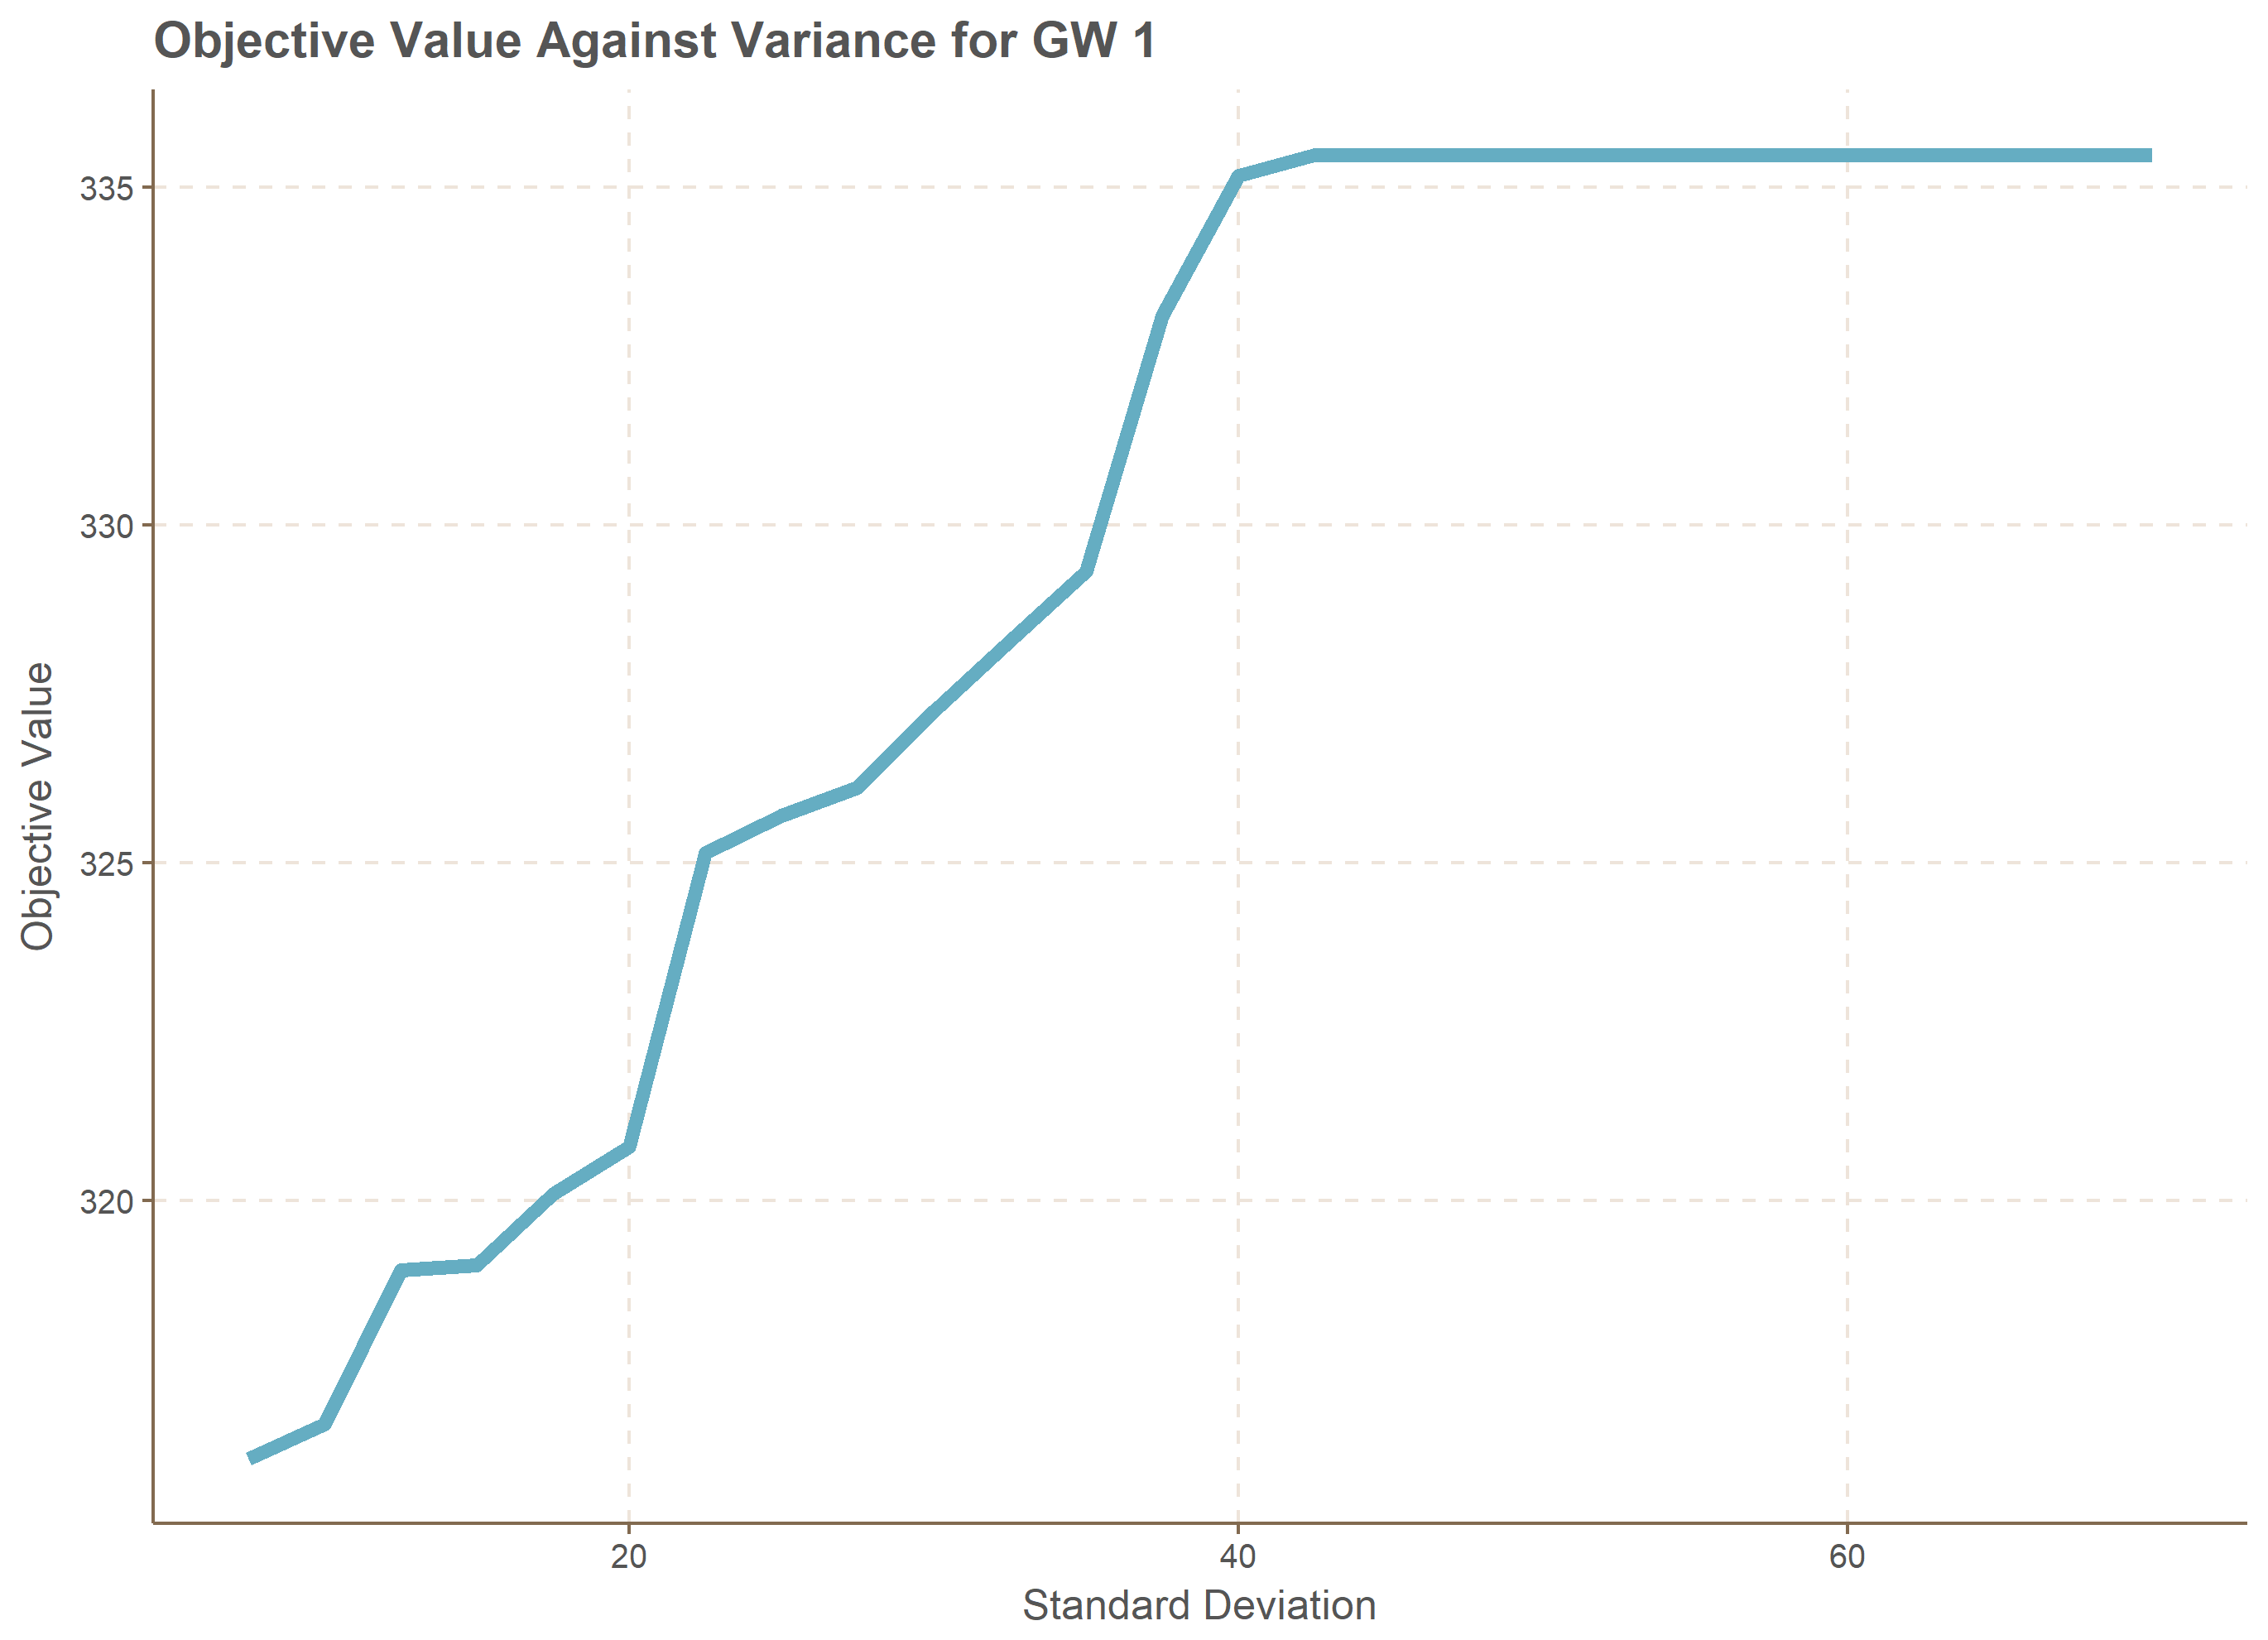
\includegraphics[scale=0.5]{fig/chapter_7/GW1_var.png}
    \caption{Threshold plotted against objective value in the mathematical model.}
\label{fig:threshold_GW1}    
\end{figure}%


In Figure \ref{fig:performance_varying_threshold}, the mean points of the 2017/2018 season is plotted for different thresholds. Due to computational difficulties in the software, Mosel Xpress-MP, the model was stopped when a solution within 2 \% optimality gap was found. From Figure \ref{fig:performance_varying_threshold}, it is observable that the plot deviates from that of the efficient frontier, but some similarities can be found. Higher thresholds are for instance associated with higher mean scores, and lower thresholds are associated with lower mean scores. Note, however, that a portfolio's return does not necessarily follow the efficient frontier when an analysis of realized returns is performed.

\newpar

It is worth noting that when the constraint is not binding, the mean stabilizes at 54.3 points. Intuitively, the mean should have been that same as without the constraints. However, after examining the objective values, it is clear that there are different solutions with the same expected value for each run in gameweek 1. Thus, there is no guarantee that the solver selects the same solution. A possible way around is a different implementation of variance constraints. A \textit{trade-off approach} \citep{Speranza} is an interesting alternative, where instead of bounding the variance it is rather taken into consideration by moving it to the objective function. However, as the difference in terms of mean is small, this is not considered a major issue.

\begin{figure}[H]
    \centering
    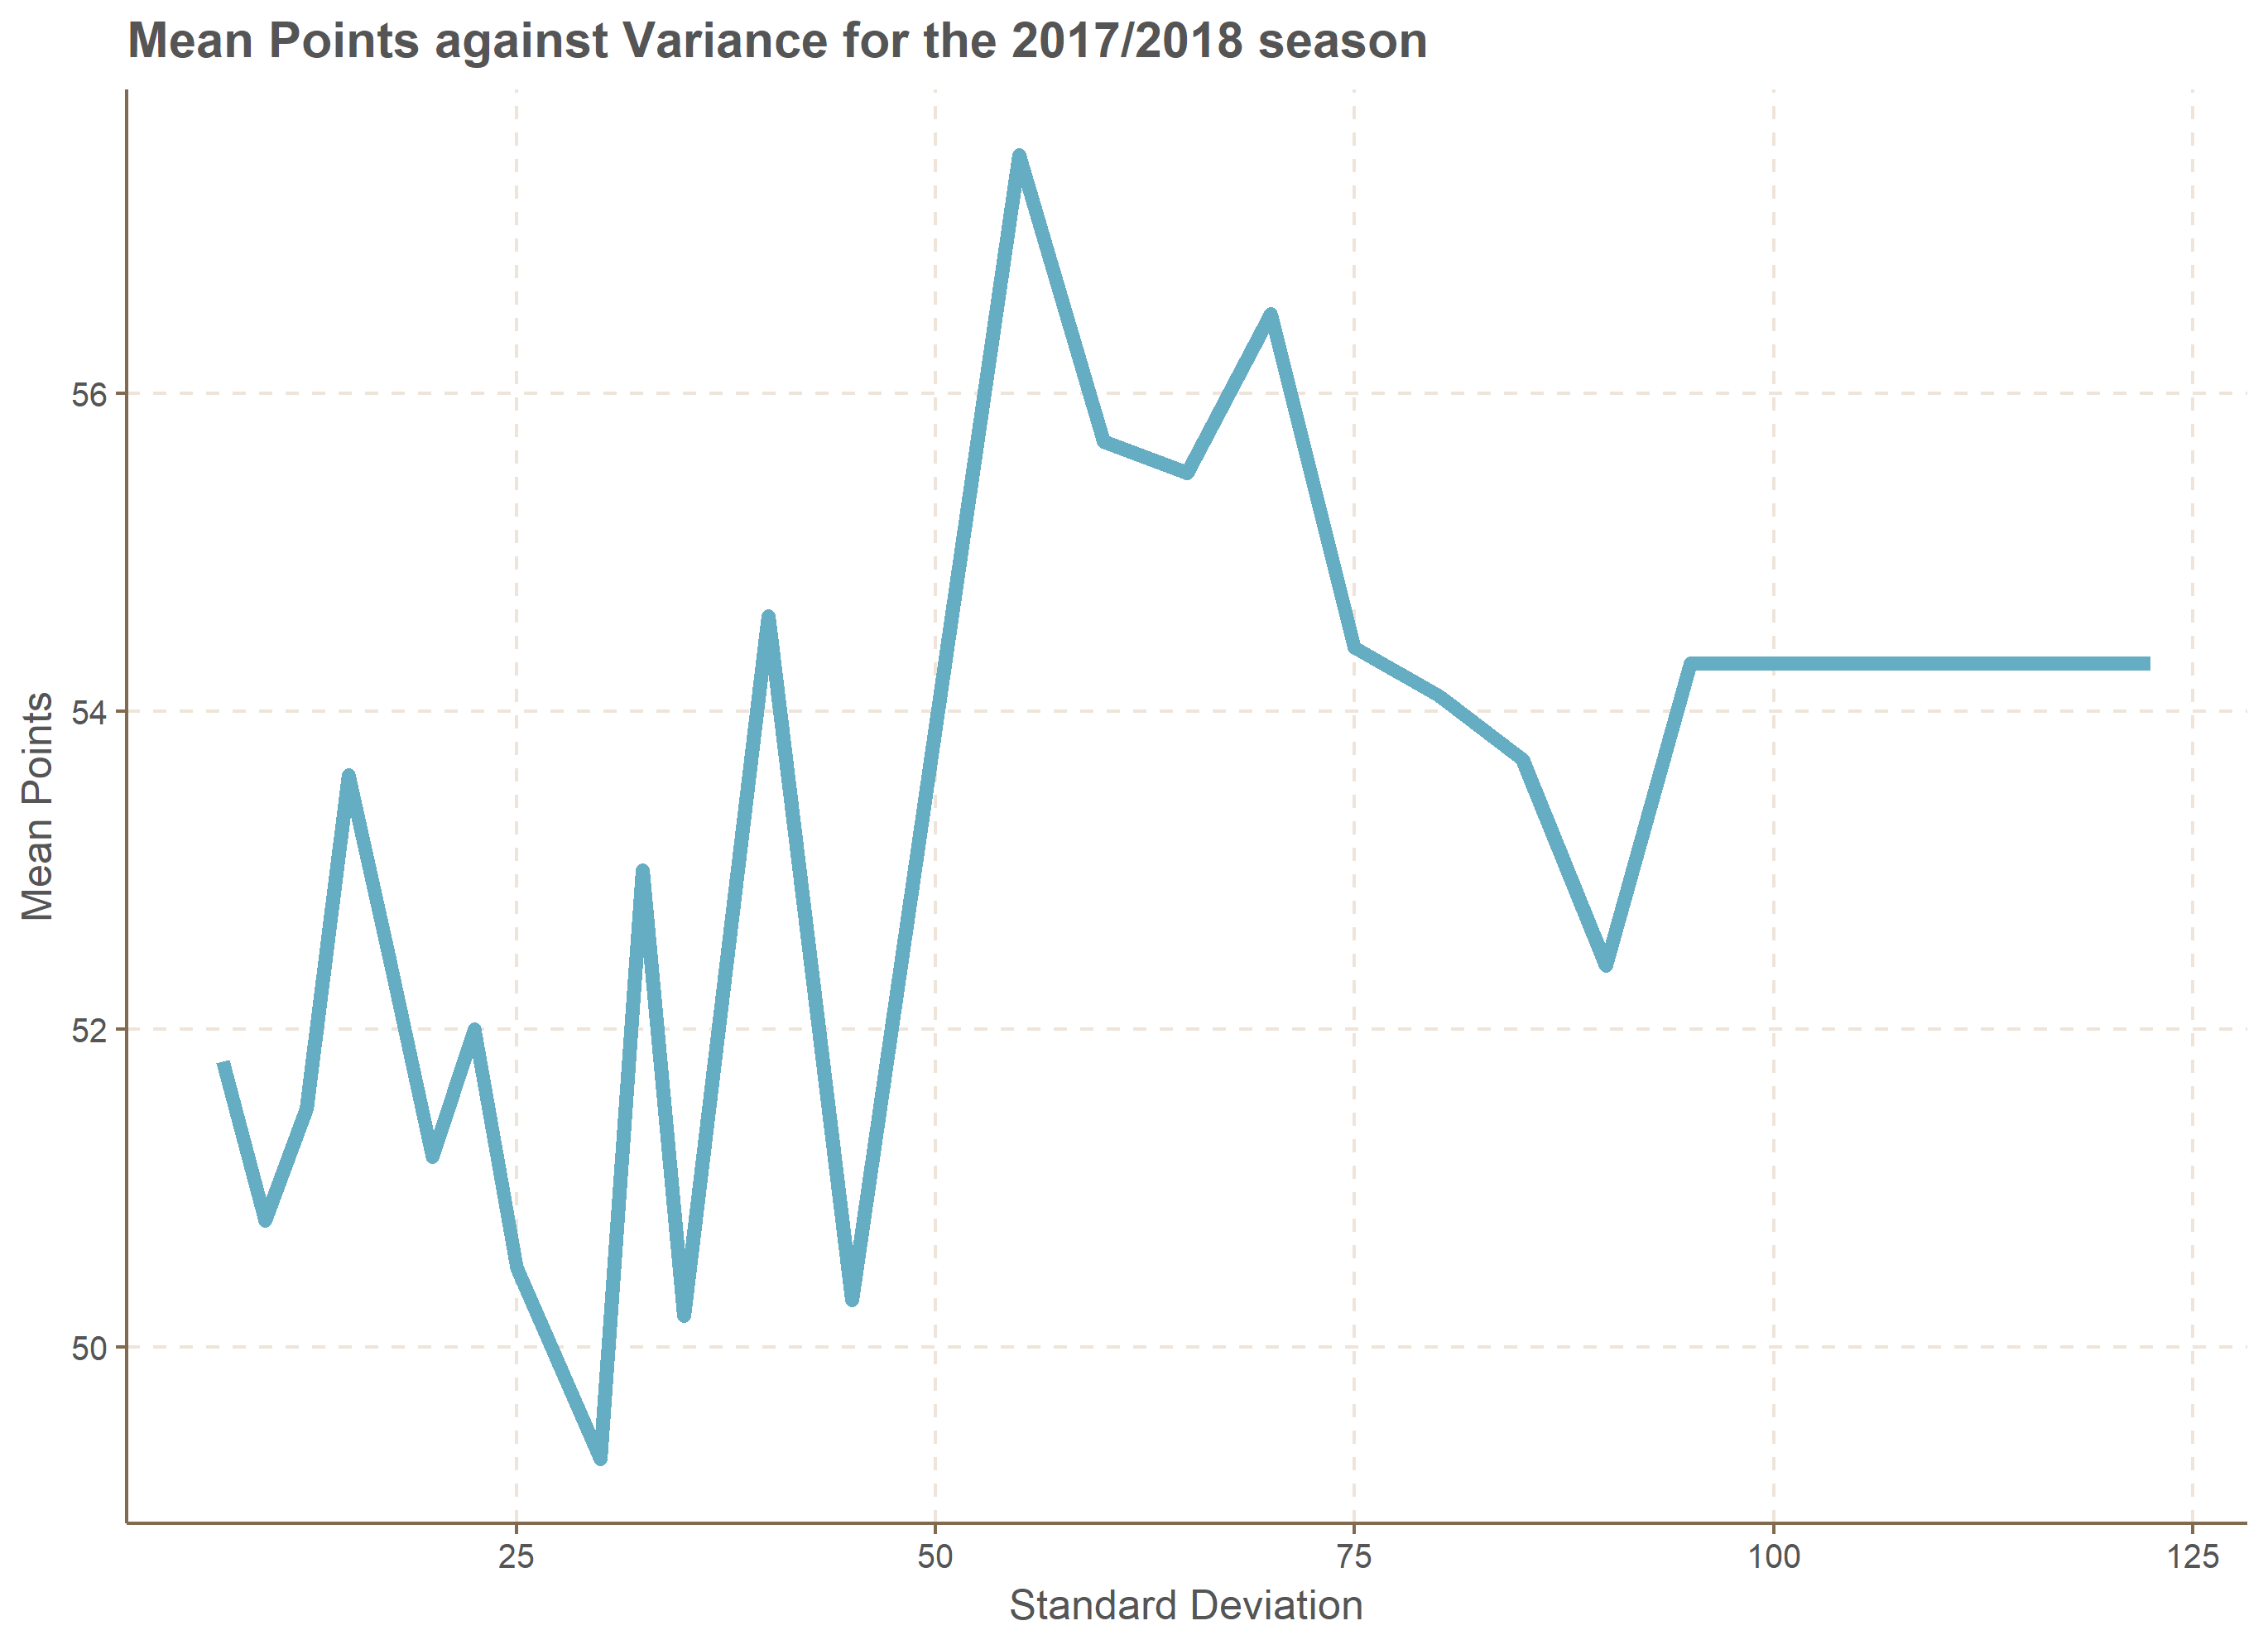
\includegraphics[scale=0.5]{fig/chapter_7/var.png}
    \caption{Results of the performance when varying threshold.}
\label{fig:performance_varying_threshold}    
\end{figure}%


As seen in Figure \ref{fig:performance_varying_threshold}, the best mean score is not reached for an unlimited threshold, but for a standard deviation of 55 points. For this point, the method would have achieved mean of 57.5? points, earning a spot among the top 1.5\%. Furthermore, in the area with a standard deviation between 55-70 points, the solutions outperform the solution with an unlimited threshold. Moreover, in the area of a standard deviation between 7.5 and 15 points, the mean score is lower than that of the unlimited case. 

\begin{figure}[H]
    \centering
    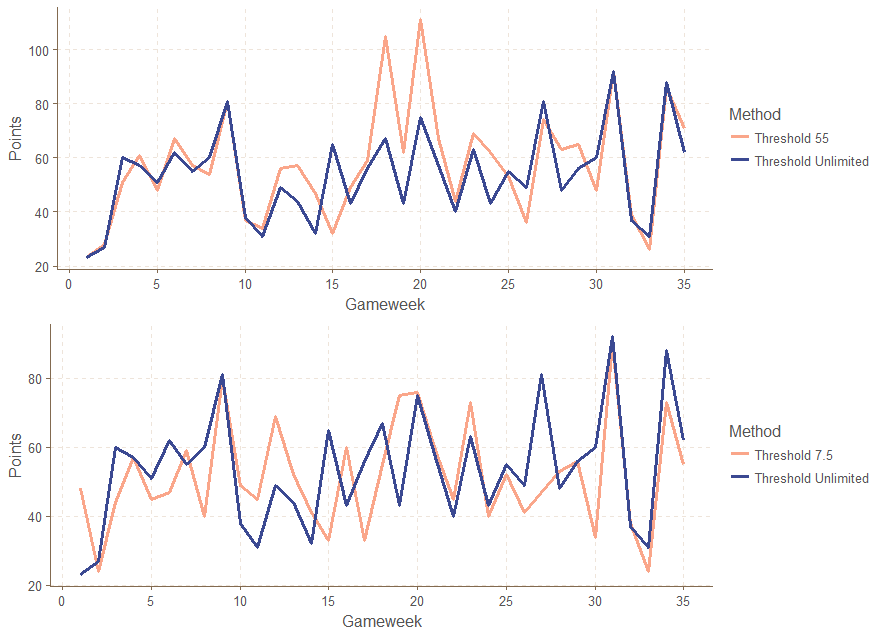
\includegraphics[scale=0.5]{fig/chapter_7/var_threshold.png}
    \caption{Plot of the results with $\sigma_0^{2} = 55^2$ and without variance constraints.}
\label{fig:performance_different_threshold}    
\end{figure}%
\newpar

In Figure \ref{fig:performance_different_threshold}, the solutions with threshold 55 and 7.5 are plotted against the solution without a variance threshold. It is noticeable that the variance appears to be higher than for the unlimited case when the threshold is 55, but not 7.5. In Table \ref{tab_high_low_thresholds}, the mean, and standard deviation for thresholds 7.5-15 and 55-70 are shown. Based on the table, it is clear that the goal of achieving lower variance in the solution is reached with lower thresholds. However, the mean is reduced, analogous to the case of portfolio optimization. Furthermore, the variance for the thresholds in the region 55-70 exceeds the variance of the unlimited case. Observe that when the thresholds are between 7.5-15, even if the thresholds lower variance, there is a mismatch between the thresholds and the realized standard deviations. For threshold between 55-70, however, the standard deviation is well below the threshold. Yet, as the threshold is approximately as high as the mean points obtained, it can be argued that it is counter intuitive that such a threshold should be binding.

\begin{table}[H]
\centering
\begin{tabular}{@{}lcc@{}}
\toprule
Threshold & Mean & St.dev \\ \midrule
7.5       & 51.7 & 15.7   \\
10        & 50.7 & 14.6   \\        %Mean = 51.9
12.5      & 51.5 & 15.9   \\
15        & 53.6 & 17.1   \\
Unlimited & 53.7 & 16.8   \\
55        & 57.5 & 20.8   \\
60        & 55.7 & 18.1   \\
65        & 55.5 & 18.8   \\
70        & 56.5 & 17.4   \\ \bottomrule 
\end{tabular}
\caption{Results for the high and low thresholds.}
\label{tab_high_low_thresholds}
\end{table}

\newpar

To summarize, threshold between 55-70 points appears to have a positive effect on performance in terms of mean, but not in terms of stabilizing points. Furthermore, a threshold of 7.5-15 points appears to be able to lower variance at the cost of mean obtained. An interval where both the standard deviation is decreased, and the performance is increased, is not found. Again, we stress that all results are based on data of two seasons and are indicative at best.







\newpar



\begin{comment}
In the end, it is interesting to investigate how different the teams actually are with the introduction of variance constraints. Do the model choose players which are stable and always achieves a certain amount of points? And, do the model choose players which plays for opposing teams? Or the model always try to pick players which do not play against each other? In general, do the behaviour of the model imitate the analogy of diversification in portfolio management? If so, this is a great finding. 
\end{comment}







\begin{comment}

\begin{table}[H]
\centering
\begin{tabular}{@{}lll@{}}
\toprule
$\sigma^2$ & Expected Points GW1 & Computational Time (seconds) \\ \midrule
$5^2$       & 314.185              & 315.917            \\
$7.5^2$     & 317.951             & 207.44             \\
$10^2$      & 318.84              & 919.085            \\
$12.5^2$    & 318.759             & 140.888            \\
$15^2$      & 319.619             & 1005.57            \\
$17.5^2$    & 322.155             & 183.62             \\
$20^2$       & 323.391             & 848.809            \\
$22.5^2$ & 324.712             & 103.374            \\
$25^2$       & 327.164             & 685.687            \\
$27.5^2$& 325.11              & 140.167            \\
$30^2$       & 327.445             & 590.303            \\
$32.5^2$     & 330.43              & 116.318            \\
$35^2$      & 329.316             & 629.958            \\
$37.5^2$     & 333.1               & 82.781             \\
$40^2$      & 335.164             & 105.532            \\
$42.5^2$    & 335.475             & 27.688             \\
$45^2$      & 335.475             & 102.61             \\
$47.5^2$    & 335.475             & 27.403             \\
$50^2$      & 335.475             & 103.023            \\
$52.5^2$    & 335.475             & 27.621             \\
$55^2$      & 335.475             & 94.686             \\
$57.5^2$     & 335.475             & 27.382             \\
$60^2$      & 335.475             & 86.712             \\
$62.5^2$     & 335.475             & 27.5               \\
$65^2$      & 335.475             & 65.378             \\
$67.5^2$    & 335.475             & 21.747             \\
$70^2$      & 335.475             & 102.856            \\
$72.5^2$     & 335.475             & 27.775             \\
$75^2$      & 335.475             & 169.981            \\
$77.5^2$    & 335.475             & 27.752             \\
$80^2$      & 335.475             & 118.392            \\
$82.5^2$    & 335.475             & 27.619             \\
$85^2$      & 335.475             & 111.9              \\
$87.5^2$    & 335.475             & 27.589             \\
$90^2$      & 335.475             & 128.027            \\
$92.5^2$    & 335.475             & 27.612             \\
$95^2$      & 335.475             & 114.051            \\
$97.5^2$    & 335.475             & 27.627             \\
$100^2$     & 335.475             & 109.042            \\ \bottomrule
\end{tabular}
\caption{Expected points GW1 run with different thresholds}
\label{tab: threshold_expected_points_gw1}
\end{table}

\end{comment}

\begin{comment}

\begin{table}[H]
\centering
\begin{tabular}{@{}lll@{}}
\toprule
$\sigma^2$ & Expected Points GW1 & Computational Time (seconds) \\ \midrule
$5^2$      & 316.497             & 237.922                      \\
$7.5^2$    & 316.177             & 222.871                      \\
$10^2$     & 316.688             & 229.821                      \\
$12.5^2$   & 318.966             & 212.807                      \\
$15^2$     & 319.036             & 199.863                      \\
$17.5^2$   & 320.095             & 169.172                      \\
$20^2$     & 320.795             & 208.512                      \\
$22.5^2$   & 325.147             & 150.152                      \\
$25^2$     & 325.69              & 128.731                      \\
$27.5^2$   & 325.155             & 175.345                      \\
$30^2$     & 327.236             & 114.991                      \\
$32.5^2$   & 328.283             & 135.686                      \\
$35^2$     & 329.316             & 160.517                      \\
$37.5^2$   & 333.1               & 84.139                       \\
$40^2$     & 335.164             & 36.723                       \\
$42.5^2$   & 335.475             & 27.879                       \\
$45^2$     & 335.475             & 28.255                       \\
$47.5^2$   & 335.475             & 27.94                        \\
$50^2$     & 335.475             & 27.67                        \\
$52.5^2$   & 335.475             & 27.9                         \\
$55^2$     & 335.475             & 28.264                       \\
$57.5^2$   & 335.475             & 28.517                       \\
$60^2$     & 335.475             & 27.852                       \\
$62.5^2$   & 335.475             & 28.239                       \\
$65^2$     & 335.475             & 21.667                       \\
$67.5^2$   & 335.475             & 21.829                       \\
$70^2$     & 335.475             & 28.004                       \\
$72.5^2$   & 335.475             & 29.227                       \\
$75^2$     & 335.475             & 28.512                       \\
$77.5^2$   & 335.475             & 28.68                        \\
$80^2$     & 335.475             & 28.372                       \\
$82.5^2$   & 335.475             & 28.581                       \\
$85^2$     & 335.475             & 28.831                       \\
$87.5^2$   & 335.475             & 29.032                       \\
$90^2$     & 335.475             & 27.962                       \\
$92.5^2$   & 335.475             & 27.613                       \\
$95^2$     & 335.475             & 28.242                       \\
$97.5^2$   & 335.475             & 28.411                       \\
$100^2$    & 335.475             & 28.626                       \\ \bottomrule
\end{tabular}
\caption{Expected points GW1 run with different thresholds}
\label{tab: threshold_expected_points_gw1}
\end{table}

\end{comment}



\begin{comment}

\begin{table}[]
\centering
\begin{tabular}{@{}lll@{}}
\toprule
Threshold & Expected Points GW1 & Computational Time \\ \midrule
56.25     & 317.951             & 207.44             \\
156.25    & 318.759             & 140.888            \\
306.25    & 322.155             & 183.62             \\
506.25    & 324.712             & 103.374            \\
756.25    & 325.11              & 140.167            \\
1056.25   & 330.43              & 116.318            \\
1406.25   & 333.1               & 82.781             \\
1806.25   & 335.475             & 27.688             \\
2256.25   & 335.475             & 27.403             \\
2756.25   & 335.475             & 27.621             \\
3306.25   & 335.475             & 27.382             \\
3906.25   & 335.475             & 27.5               \\
4556.25   & 335.475             & 21.747             \\
5256.25   & 335.475             & 27.775             \\
6006.25   & 335.475             & 27.752             \\
6806.25   & 335.475             & 27.619             \\
7656.25   & 335.475             & 27.589             \\
8556.25   & 335.475             & 27.612             \\
9506.25   & 335.475             & 27.627             \\ \bottomrule
\end{tabular}
\caption{Expected points GW1 run with different thresholds}
\label{tab: threshold_expected_points_gw1_halves}
\end{table}


\end{comment}



\begin{comment}


- hvis man plotter threshold opp mot perfekt poeng burde man ikke få en rett strek, men man skulle forvente en synkende trend ved synkende threshold 

- hvor annerledes er selve laget når man inkluderer threshold - ved hvilket threshold begynner laget å bli annerledes fra uten threshold?

- viktig å understreke at dette kun er en realisering av poeng og man ikke kan trekke generelle konklusjoner, men det er allikevel nyttig å gjøre en analyse for å få innblikk i dens påvirkning. 

- hva vil det si at man adder threshold, jo at manager har en risk profil som karakteriseres mellom risk-taking, risk-neutral og risk-averse 

- å adde risk kan være en add-on i forhold til hvilke risk profil en manager kan ha. det kan være at en manager er opptatt av å kun ha et stabilt lag og ikke ta så mye risk. da kan varians constraints være en kjempe add-on

-med for lave threshold skulle man tro at problemet ble vanskelig å løse siden alle har en positiv varians, men kan være den velger spiller med størst negativ korrelasjon mellom dem for å holde threshold constraints. 


\end{comment}
